\documentclass[12pt]{iopart}

\usepackage[activate={true, nocompatibility}, final, tracking=true, kerning=true, spacing=true, factor=1100, stretch=10, shrink=10]{microtype}
\microtypecontext{spacing=nonfrench}

\usepackage[pdftex]{graphicx}
\usepackage[caption=false]{subfig}

\usepackage{siunitx}
\usepackage[ruled, linesnumbered]{algorithm2e}
\DontPrintSemicolon

\usepackage[acronym, nomain]{glossaries}

\newacronym{13N-NH3}{[$^{13}$N]-NH$3$}{Nitrogen-$13$ Ammonia}
\newacronym{18F-FDG}{[$^{18}$F]-FDG}{Fluorine-$18$ Fludeoxyglucose}
\newacronym{1D}{$1$D}{One Dimensional}
\newacronym{2D}{$2$D}{Two Dimensional}
\newacronym{3D}{$3$D}{Three Dimensional}
% \newacronym{3DPC}{3DPC}{Three Dimensional Point Cloud}
\newacronym{4D}{$4$D}{Four Dimensional}
\newacronym{4DCT}{$4$DCT}{Four Dimensional Computed Tomography}
\newacronym{ACF}{ACF}{Attenuation Correction Factor}
\newacronym{AC}{AC}{Attenuation Corrected}
% \newacronym{AD}{AD}{Affine Deformation}
\newacronym{AE}{AE}{Autoencoder}
\newacronym{AIF}{AIF}{Arterial Input Function}
\newacronym{AI}{AI}{Artificial Intelligence}
\newacronym{ALS}{ALS}{Amyotrophic Lateral Sclerosis}
\newacronym{APD}{APD}{Avalanche Photodiode}
\newacronym{AP}{AP}{Anterior Posterior}
\newacronym{ATP}{ATP}{Adenosine Triphosphate}
\newacronym{AUC}{AUC}{Area Under the Curve}
\newacronym{AV-CCT}{AV-CCT}{Averaged CINE-Computed Tomography}
% \newacronym{BE}{BE}{Bending Energy}
\newacronym{BFGS}{BFGS}{Broyden Fletcher Goldfarb Shanno}
\newacronym{BGO}{BGO}{Bismuth Germanium Oxide}
\newacronym{BP}{BP}{Back Projection}
\newacronym{CC}{CC}{Correlation Coefficient}
\newacronym{CCT}{CCT}{CINE-Computed Tomography}
\newacronym{CCP}{CCP}{Collaborative Computational Project}
\newacronym{CDT}{CDT}{Centre for Doctoral Training}
\newacronym{CF}{CF}{Clinical Features}
% \newacronym{CG}{CG}{Conjugate Gradient}
\newacronym{CLBP}{CLBP}{Chronic Low Back Pain}
\newacronym{CNN}{CNN}{Convolutional Neural Network}
\newacronym{CMR}{CMR}{CINE-Magnetic Resonance}
\newacronym{COD}{COD}{Centroid of Distribution}
\newacronym{COM}{COM}{Centre of Mass}
\newacronym{CP}{CP}{Control Point}
\newacronym{CPG}{CPG}{Control Point Grid}
\newacronym{CT}{CT}{Computed Tomography}
\newacronym{CV}{nCV}{Normalised Coefficient of Variance}
\newacronym{DDG}{DDG}{Data Driven Gating}
\newacronym{DD-PCA}{DD-PCA}{Data Driven Principal Component Analysis Surrogate Signal Extraction}
\newacronym{DD}{DD}{Data Driven}
\newacronym{DIP}{DIP}{Deep Image Prior}
\newacronym{DVF}{DVF}{Deformation Vector Field}
\newacronym{DWB}{DWB}{Dynamic Whole Body}
\newacronym{EANM}{EANM}{European Association of Nuclear Medicine}
\newacronym{EC}{EC}{Event Conditional}
\newacronym{ELU}{ELU}{Exponential Linear Unit}
\newacronym{EM}{EM}{Expectation Maximisation}
\newacronym{EPSRC}{EPSRC}{Engineering and Physical Sciences Research Council}
\newacronym{FBP}{FBP}{Filtered Back Projection}
\newacronym{FDG}{FDG}{Fluorodeoxyglucose}
\newacronym{FFT}{FFT}{Fast Fourier Transform}
\newacronym{FOV}{FOV}{Field of View}
\newacronym{FWHM}{FWHM}{Full Width at Half Maximum}
\newacronym{GAN}{GAN}{Generative Adversarial Networks}
\newacronym{GD}{GD}{Gradient Descent}
\newacronym{GE}{GE}{General Electric}
\newacronym{GPU}{GPU}{Graphics Processing Unit}
\newacronym{Grad-CAM}{Grad-CAM}{Gradient-weighted Class Activation Mapping}
% \newacronym{GT}{GT}{Ground Truth}
\newacronym{HAB}{HAB}{High Affinity Binder}
% \newacronym{HC}{HC}{Healthy Control}
\newacronym{HPLC}{HPLC}{High Performance Liquid Chromatography}
\newacronym{HU}{HU}{Hounsfield Unit}
\newacronym{i4health}{i$4$health}{Intelligent, Integrated Imaging in Healthcare}
\newacronym{IDIF}{IDIF}{Image Derived Input Function}
\newacronym{IF}{IF}{Input Function}
\newacronym{ILD}{ILD}{Interstitial Lung Disease}
\newacronym{IPF}{IPF}{Idiopathic Pulmonary Fibrosis}
% \newacronym{IR}{IR}{Image Registration}
\newacronym{KBq/mL}{KBq/mL}{Kilo Becquerel per Millilitre}
\newacronym{KeV}{KeV}{Kiloelectron Volt}
\newacronym{KLD}{KLD}{Kullback Leibler Deviation}
\newacronym{KO}{KO}{Knee Osteoarthritis}
\newacronym{KRG}{KRG}{Kinetic Respiratory Gating}
\newacronym{KV}{KV}{Kilo Volt}
\newacronym{L-BFGS-B}{L-BFGS-B}{Low memory Broyden Fletcher Goldfarb Shanno Bounded}
\newacronym{L-BFGS}{L-BFGS}{Low memory Broyden Fletcher Goldfarb Shanno}
\newacronym{LED}{LED}{Light Emitting Diode}
% \newacronym{LE}{LE}{Linear Energy}
% \newacronym{LL}{LL}{Log Likelihood}
\newacronym{LM}{LM}{Lateral Medial}
\newacronym{LOR}{LOR}{Line of Response}
% \newacronym{LR}{LR}{Linear Regression}
\newacronym{LSO}{LSO}{Lutetium Oxyorthosilicate}
\newacronym{LSTM}{LSTM}{Long Short Term Memory}
\newacronym{LYSO}{LYSO}{Lutetium Yttrium Orthosilicate}
\newacronym{NIHR}{NIHR}{National Institute for Health Research}
\newacronym{MAB}{MAB}{Mixed Affinity Binder}
\newacronym{MAD}{MAD}{Median Absolute Difference}
\newacronym{MAE}{MAE}{Mean Absolute Error}
\newacronym{MAPE}{MAPE}{Mean Absolute Percentage Error}
% \newacronym{MBF}{MBF}{Myocardial Blood Flow}
\newacronym{MB}{MB}{Memory Bank}
\newacronym{MCIR}{MCIR}{Motion Compensated Image Reconstruction}
% \newacronym{MCI}{MCI}{Motion Compensated Image}
\newacronym{mCi}{mCi}{Millicurie}
% \newacronym{MC}{MC}{Motion Correction}
\newacronym{MeV}{MeV}{Megaelectron Volt}
\newacronym{MIC}{MIC}{Medical Imaging Convention}
\newacronym{MI}{MI}{Mutual Information}
\newacronym{MLAA}{MLAA}{Maximum Likelihood Reconstruction of Activity and Attenuation}
\newacronym{MLACF}{MLACF}{Maximum Likelihood Activity and Attenuation Correction Factors Estimation}
\newacronym{MLEM}{MLEM}{Maximum Likelihood Expectation Maximisation}
% \newacronym{MLE}{MLE}{Maximum Likelihood Estimation}
% \newacronym{ML}{ML}{Machine Learning}
\newacronym{ML}{ML}{Maximum Likelihood}
\newacronym{MM}{MM}{Motion Model}
\newacronym{MNI}{MNI}{Montreal Neurological Institute}
% \newacronym{MPI}{MPI}{Myocardial Perfusion Imaging}
\newacronym{MR}{MR}{Magnetic Resonance}
\newacronym{MSc}{MSc}{Master of Science}
\newacronym{MSE}{MSE}{Mean Squared Error}
\newacronym{Mu-Map}{$\mu$-Map}{Attenuation Map}
\newacronym{NAC}{NAC}{Non-Attenuation Corrected}
\newacronym{NaI(Ti)}{NaI(Ti)}{Sodium Iodide Thallium}
\newacronym{NaN}{NaN}{Not a Number}
\newacronym{NMI}{NMI}{Normalised Mutual Information}
\newacronym{ND}{ND}{$n$-Dimensional}
\newacronym{NLP}{NLP}{Natural Language Processing}
% \newacronym{Non-MC}{Non-MC}{Non-Motion Corrected}
\newacronym{NN}{NN}{Neural Network}
% \newacronym{Non-RD}{Non-RD}{Non-Rigid Deformation}
\newacronym{Non-TOF}{Non-TOF}{Non-Time of Flight}
\newacronym{OSEM}{OSEM}{Ordered Subset Expectation Maximisation}
\newacronym{OSIC}{OSIC}{Open Source Imaging Consortium}
\newacronym{PBR28}{[$^{11}$C]-PBR$28$}{[$^{11}$C]-Peripheral Benzodiazepine Receptor}
\newacronym{PC}{PC}{Principal Component}
\newacronym{PCA}{PCA}{Principal Component Analysis}
\newacronym{PET}{PET}{Positron Emission Tomography}
\newacronym{PIQE}{PIQE}{Perception Based Image Quality Evaluator}
% \newacronym{PLL}{PLL}{Poisson Log Likelihood}
\newacronym{PMT}{PMT}{Photomultiplier Tube}
\newacronym{PReLU}{PReLU}{Parametric Rectified Linear Unit}
\newacronym{PSD}{PSD}{Power Spectral Density}
\newacronym{PSMA}{PSMA}{Prostate Specific Membrane Antigen}
% \newacronym{PT}{PT}{Patient}
\newacronym{RAE}{RAE}{Relative Absolute Error}
\newacronym{RANSAC}{RANSAC}{Random Sample Consensus}
\newacronym{RCM}{RCM}{Respiratory Correspondence Model}
% \newacronym{RD}{RD}{Rigid Deformation}
\newacronym{RDP}{RDP}{Relative Difference Prior}
\newacronym{ReLU}{ReLU}{Rectified Linear Unit}
% \newacronym{RM}{RM}{Respiratory Motion}
% \newacronym{RMC}{RMC}{Respiratory Motion Correction}
\newacronym{RMSE}{RMSE}{Root Mean Square Error}
\newacronym{ROI}{ROI}{Region of Interest}
\newacronym{RPM}{RPM}{Real Time Position Management}
\newacronym{SAM}{SAM}{Spectral Analysis Method}
\newacronym{SELU}{SELU}{Scaled Exponential Linear Unit}
\newacronym{SGD}{SGD}{Stochastic Gradient Descent}
\newacronym{SiPM}{SiPM}{Silicon Photomultiplier}
\newacronym{SIRF}{SIRF}{Synergistic Image Reconstruction Framework}
\newacronym{SI}{SI}{Superior Inferior}
\newacronym{SNR}{SNR}{Signal to Noise Ratio}
\newacronym{SPECT}{SPECT}{Single-photon Emission Computed Tomography}
\newacronym{SRF}{SRF}{Sinogram Region Fluctuation}
\newacronym{SS}{SS}{Surrogate Signal}
\newacronym{SSD}{SSD}{Sum of Squared Differences}
\newacronym{SSIM}{SSIM}{Structural Similarity Index Measure}
\newacronym{SSPM}{SSPM}{Solid State Photomultiplier}
\newacronym{STD}{STD}{Standard Deviation}
\newacronym{STFT}{STFT}{Short Time Fourier Transform}
\newacronym{STIR}{STIR}{Software for Tomographic Image Reconstruction}
\newacronym{SuPReMo}{SuPReMo}{Surrogate Parametrised Respiratory Motion Modelling}
\newacronym{SUV}{SUV}{Standard Uptake Value}
\newacronym{SVD}{SVD}{Singular Value Decomposition}
\newacronym{SyneRBI}{SyneRBI}{Synergistic Biomedical Imaging}
\newacronym{TAC}{TAC}{Time Activity Curve}
\newacronym{TCM}{TCM}{Tissue Compartment Model}
\newacronym{TOF}{TOF}{Time of Flight}
% \newacronym{TPS}{TPS}{Thin Plate Spline}
\newacronym{TSPO}{TSPO}{Translocator Protein $18$ kDa}
\newacronym{TV}{TV}{Total Variation}
\newacronym{UCLH}{UCLH}{University College London Hospitals}
\newacronym{UCL}{UCL}{University College London}
\newacronym{UK}{UK}{United Kingdom}
\newacronym{VOI}{VOI}{Volume of Interest}
\newacronym{VT}{V$_{\mathrm{T}}$}{Volume of Distribution}
\newacronym{XCAT}{XCAT}{Four Dimensional Extended Cardiac Torso}


\usepackage[style=authoryear, backend=biber, mincitenames=1, maxcitenames=2, minbibnames=1, maxbibnames=99, uniquelist=false, uniquename=false]{biblatex}
\addbibresource{./Biblio.bib}

\begin{document}
    \title[Data driven surrogate signal extraction for dynamic PET using selective PCA]{Data driven surrogate signal extraction for dynamic PET using selective PCA: time windows versus the combination of components}
    
    % \author{Alexander~C~Whitehead$^{1, 2, 3}$, Kuan-Hao~Su$^4$, Elise~C~Emond$^1$, Ander~Biguri$^5$, Ludovica~Brusaferri$^6$, Maria~Machado$^1$, Joanna~C~Porter$^7$, Helen~Garthwaite$^7$, Scott~D~Wollenweber$^4$, Jamie~R~McClelland$^2$ and Kris~Thielemans$^{1, 2}$}
    
    % \address{$^1$ Institute of Nuclear Medicine, University College London, UK}
    % \address{$^2$ Centre for Medical Image Computing, University College London, UK}
    % \address{$^3$ Department of Computer Science, University College London, UK}
    % \address{$^4$ Molecular Imaging and Computed Tomography Engineering, GE Healthcare, USA}
    % \address{$^5$ Department of Applied Mathematics and Theoretical Physics, University of Cambridge, UK}
    % \address{$^6$ Computer Science and Informatics, London South Bank University, UK}
    % \address{$^7$ Centre for Respiratory Medicine, University College London, UK}
    
    % \ead{alexander.whitehead.18@ucl.ac.uk}
    
    \begin{abstract}
        \paragraph{Objective} Respiratory motion correction is beneficial in PET, as it can reduce artefacts caused by motion and improve quantitative accuracy. Methods of motion correction are commonly based on a respiratory trace obtained through an external device (like the Real Time Position Management System) or a data driven method, such as those based on dimensionality reduction techniques (for instance PCA). PCA itself being a linear transformation to the axis of greatest variation. Data driven methods have the advantage of being non-invasive, and can be performed post-acquisition. However, their main downside being that they are adversely affected by the tracer kinetics of the dynamic PET acquisition. Therefore, they are mostly limited to static PET acquisitions. This work seeks to extend on existing PCA-based data-driven motion correction methods, to allow for their applicability to dynamic PET imaging.
        \paragraph{Approach} The methods explored in this work include; a moving window approach (similar to the Kinetic Respiratory Gating method from Schleyer et al.), extrapolation of the principal component from later time points to earlier time points, and a method to score, select, and combine multiple respiratory components. The resulting respiratory traces were evaluated on $22$ data sets from a dynamic ${}^{18F}$FDG study on patients with Idiopathic Pulmonary Fibrosis. This was achieved by calculating their correlation with a surrogate signal acquired using a Real Time Position Management System.
        \paragraph{Main results} The results indicate that all methods produce better surrogate signals than when applying conventional PCA to dynamic data (for instance, a higher correlation with a gold standard respiratory trace). Extrapolating a late time point principal component produced more promising results than using a moving window. Scoring, selecting, and combining components held benefits over all other methods.
        \paragraph{Significance} This work allows for the extraction of a surrogate signal from dynamic PET data earlier in the acquisition and with a greater accuracy than previous work. This potentially allows for numerous other methods (for instance, respiratory motion correction) to be applied to this data (when they otherwise could not be previously used).
    \end{abstract}
    
    \noindent{\it Keywords\/}: PET, Dynamic PET, Surrogate Signal Extraction, PCA, Data Driven Gating
    
    \submitto{\PMB}
    
    \maketitle
    
    \section{Introduction} \label{sec:introduction}
    Respiratory motion reduces image resolution by introducing blurring as well as misalignment artefacts in \gls{PET}~\parencite{Nehmeh2008a}. Methods of motion correction, such as gating, are commonly based on a surrogate signal, see~\parencite{Lamare2022PETVadis, Kyme2021MotionCT} for recent reviews. This surrogate signal is a respiratory trace which reflects the position of the anatomy of the patient in the respiratory cycle over time~\parencite{Kesner2010AMethods, Kesner2013GatingPET}.
    
    Initial research concentrated on methods that determine the surrogate signal via an external device, for instance, a spirometer~\parencite{Voscopoulos2013EvaluationScenarios}, a belt~\parencite{Yu2016}, or an imaging device such as a depth sensing camera~\parencite{Silverstein2018ComparativeSensor, Xia2012AConcept}, or the \gls{RPM}~\parencite{Bettinardi2013Motion-trackingPET/CT}. However, using external devices suffers from several disadvantages, such as  drift and/or requiring a constant line of sight. Furthermore, most external device methods can only track the surface deformations of the patient, as opposed to the internal ones. Finally, such methods require the use of additional equipment, a change to clinical practise, and must be acquired alongside any other data, not retrospectively.
    
    Thus, \gls{PET} \gls{DD} methods to extract the surrogate signal, which do not require additional equipment and can be applied retrospectively, have become an alternative for static \gls{PET} data~\parencite{Kesner2014OnFramework}. \gls{DD} methods include, but are not limited to, those which attempt to spatially track aspects of the acquisition data, be that reconstructed or not, or ones which use methods such as dimensionality reduction~\parencite{Lamare2022PETVadis}. We briefly discuss these methods here but see also section~\ref{sec:methods}.
    
    Some \gls{DD} solutions make use of aspects of the image acquisition itself, by reconstructing short time frame images and tracking regions of them over time. Such as, an external or inserted radioactive fiducial marker~\parencite{Buther2013ExternalTomography., Zimmermann2003UseMRI}, a tumour~\parencite{Bundschuh2007}, or a combination of patterns from different voxels~\parencite{Kesner2009RespiratoryData}. Some methods make use of \gls{MR} information (tracking the position of the diaphragm using a pencil shaped navigator)~\parencite{Taylor1997MRAngiography, Furst2015MotionPET/MR}. A disadvantage of image space based methods is computation time and potential poor quality due to low count statistics. Obviously methods which require the insertion of objects into a patient have the unnecessary side effect of causing harm to the patient. Furthermore, to make use of \gls{MR} information requires a combined \gls{PET}/\gls{MR}.
    
    Alternatively, aspects of the data in sinogram space can be individually tracked directly from the list mode data, such as the \gls{COD} or \gls{COM}~\parencite{Klein2001Fine-scaleInformation, Bruyant2002CorrectionPhantom, Ren2017Data-drivenDistribution, Feng2018Self-gating:PET}. A potential disadvantage is that these methods require structures with high contrast in sinogram space. A final class of methods uses short time frame sinograms (often at low spatial resolution) and detects motion patterns in the whole sinogram. Such methods rely on the fact that, in static \gls{PET}, the main cause of (non-stochastic) change in the data is motion. The main sinogram-based methods are the \gls{SAM} method~\parencite{Schleyer2009, Schleyer2011, Schleyer2018Data-DrivenMotion}, the \gls{SRF} method~\parencite{Kesner2010AMethods} and a method based on \gls{PCA}~\parencite{Thielemans2011, Bertolli2018Data-DrivenTomography}, briefly described below.

    \begin{itemize}
        \item \gls{SAM} identifies regions in sinograms which are likely to be experiencing respiratory motion. This is achieved by analysing the frequency spectrum of the result of applying a \gls{FFT} to each bin in the sinogram. A bin which is experiencing respiratory motion will have a peak in the frequency spectrum at the frequency of the respiratory motion. Through this, areas in the sinogram which are experiencing respiratory motion are determined and the total number of counts in these regions, over time, is used to estimate a \gls{SS}~\parencite{Schleyer2009, Schleyer2011, Schleyer2018Data-DrivenMotion}.

        \item \gls{SRF} proposes to recursively combine signals from sinogram bins \gls{TAC}, using a score based on the ratio between respiratory and non-respiratory content, with a positive and negative sign in order to maximise its standard deviation~\parencite{Kesner2010AMethods}. However, a disadvantage of the use of standard deviation as the objective would be that there are many ways to increase standard deviation which are not acquiring a better respiratory trace. For instance, noise may increase the standard deviation of a signal.

        \item \gls{PCA} works similarly to \gls{SVD}, in fact most implementations of \gls{PCA} use \gls{SVD}. The goal of this method is to find linear transforms of the data such that it is projected to a space along which its axis point in the direction of greatest varience (and then second greatest variance etc). For \gls{SS} extraction \gls{PCA} is applied across a time series of sinograms. The weighting of each \gls{PC} for each time point would be the signal. Generally multiple \glspl{PC} are extracted and the one which contains the most respiratory information (determined using \gls{FFT}) is selected~\parencite{Thielemans2011, Bertolli2018Data-DrivenTomography}.
    \end{itemize}
    
    To-date, evaluations of these methods have been almost exclusively performed on static \gls{PET} data, mostly using \gls{18F-FDG}. They include comparisons with external devices (such as the \gls{RPM}), \gls{MR} navigator based surrogate signals~\parencite{Manber2015PracticalPET/MR}, as well as image quality~\parencite{Buther2020ClinicalMotion, Walker2019EvaluationImaging}. Preliminary investigations indicated that many sinogram-based methods all perform similarly~\parencite{Thielemans2013ComparisonData}.
    
    However, current \gls{DD} methods are adversely affected by the radiotracer kinetics of a dynamic acquisition, where the tracer is injected after the beginning of the scan. As an example, methods that use dimensionality reduction (such as \gls{PCA}) are hampered by the fact that at the start of the scan rapid redistribution of the radiotracer, rather than the respiratory motion, causes more variance in the data. Previously, work was performed to extend the \gls{SAM} method to be robust to radiotracer kinetics. This work proposed the use of \gls{STFT} to generate masks for \gls{SAM} (rather than a static mask for all time intervals), this was called \gls{KRG}~\parencite{Schleyer2014}. \gls{STFT} operates by splitting the data into windows and doing a \gls{FFT} on them independently. This could be approximated by windowing the data first and then performing \gls{SAM}. This method was unable to extract a usable signal at very early time intervals after tracer injection however.
    
    The aim of the current work is to propose several adaptions of the \gls{PCA} method, through which it can be used with dynamic data, and compare their performance with a method based on \gls{KRG}. The methods explored in this work include the use of a moving window, re-use of the \glspl{PC} from a later time interval to estimate the surrogate signal from earlier time intervals, and the automatic selection and combination of multiple \glspl{PC}, akin to \gls{SRF}.

    Firstly, in section~\ref{sec:methods}, the data, including train and test splits, will be introduced before moving on to the methods which are being proposed or compared. Next, in section~\ref{sec:evaluation}, a more thorough description of the data, including how it is prepared, and the evaluation methods used to compare the methods are presented. In this section we also introduce potential post-processing techniques which can be performed to \glspl{SS} to improve results generally. Followed by, in section~\ref{sec:results}, figures depicting a comparison of the methods defined in the previous section are shown and discussed. The advantages and disadvantages of the methodology of the work presented is highlighted in section~\ref{sec:discussion}. Finally, in section~\ref{sec:conclusion}, the arguments put forth are drawn together before briefly pointing out the potential future directions for the work.
    
\section{Methods} \label{sec:methods}
    Here, we briefly describe the data acquisition before describing methods that are either simple modifications of the conventional methods, based on \gls{KRG}, or use a novel method to select and combine signals. These methods can be used with \gls{SAM} but for simplicity we will refer specifically to \gls{PCA}.

    \subsection{Data Acquisition and Train/Test Split} \label{sec:data_acquisition_and_train_test_split}
        Data used was acquired from a research study with patients suffering from \gls{IPF}~\parencite{Emond2020EffectReconstruction}. $22$ dynamic \gls{18F-FDG} acquisitions, with a \gls{FOV} covering the upper lung and heart, were acquired on a \gls{GE} Discovery $710$ in list-mode. Data used in this study was from the first \SI{14}{\minute} with the acquisition starting roughly \SI{20}{\second} before injection of the radiotracer. An external surrogate signal was acquired in parallel using an \gls{RPM}~\parencite{Oh2019OptimalTreatment}.

        These $22$ acquisitions comprised of two scans each of $11$ subjects. One scan was performed before and one scan was performed some time after an intervention was performed. In this case the intervention was the administration of an anticoagulant drug. The first acquisition of each patient is called the baseline scan and the second acquisition is called the post treatment scan~\parencite{Emond2020EffectReconstruction}. Of these $22$ acquisitions only $10$ were suitable to be used as either part of the training or testing process. Five of the acquisitions could not be used as the list-mode itself could not be loaded by the software. The remaining acquisitions could not be used for either training or testing due to issues with the acquisition of the \gls{RPM}, for instance the acquired \gls{RPM} could not be synced with the list-mode. These data without \gls{RPM} could be used with the subsequent methods, just not evaluated, as can be seen in figure~\ref{fig:pca_signals}.

        To form a train and test split the data was randomly split into three training data points and eight testing data points. More than one training data point was selected to attempt to prevent overfitting on a single data point. Data points from both baseline and post treatment acquisitions were added to prevent overfitting on type of acquisition. Train data points were selected such that the same patient did not appear in both the train and test dataset to attempt to mitigate data leakage. A validation dataset was not utilised due to the low number of data points.

        For selection of hyperparameters, the method was applied the train dataset and the correlation coefficients with \gls{RPM} were computed. The mean of the three resulting correlation coefficients was maximised while varying a hyperparameter.
        
    \subsection{Conventional PCA} \label{sec:conventional_pca}
        \begin{algorithm} \label{alg:conventional_score_pseudo_code}
            \caption{Conventional Score}
            \KwData{\textit{timeSeriesSinograms}, \textit{PC}, \textit{respiratoryFrequencyWindow}}
            \KwResult{\textit{respiratoryScore}}
            \;
            \For{\textit{sinogram} in \textit{timeSeriesSinograms}}{
                \textit{respiratorySignal} append \textit{sinogram} $\times$ \textit{PC}
            }
            \;
            \textit{PSD} = absolute of \gls{FFT} on \textit{respiratorySignal}\;
            \;
            \textit{respiratoryScore} = mean value of \textit{PSD}  within \textit{respiratoryFrequencyWindow}\;
            \;
        \end{algorithm}
        
        As described above in section~\ref{sec:introduction}, \gls{PCA} is applied to the entire data set in one go as it would be if the data were from a static acquisition. The \gls{PC} containing the respiratory trace may not be the first one, generically a number of \glspl{PC} are selected and a score that maximises a signal with the appropriate respiratory features (for instance, a frequency matching the common human breathing) is selected as the \gls{SS}~\parencite{Bertolli2017}. In this implementation, when selecting from a number of \glspl{PC} the one which contains respiration, the signal which maximises the score seen in the algorithm~\ref{alg:conventional_score_pseudo_code} is used. For reference, \gls{PSD} being the result of decomposing the signal into discrete frequency bins, using \gls{FFT}, where the power is the energy at that frequency.
        
        The generic equation for calculating the weights (or signal) from the \gls{PC} and data is
            
        \begin{equation} \label{eq:pc_weights}
            W = PC \times S
        \end{equation}
            
        \noindent where in equation~\ref{eq:pc_weights} $PC$ represents the \gls{PC} (which in this case is the shape of one sinogram) and $S$ represents a time series of sinograms. $\times$ denotes element-wise multiplication of the arrays (in this case multiplication of the one \gls{PC} by each sinogram in the time series $S$), followed by summing. In fact, a similar equation is used by \gls{SAM}, where a `signed mask' is multiplied with the data and summed.
            
    \subsection{Moving Window Method} \label{sec:moving_window_method}
        \begin{figure}
            \centering
            
            \includegraphics[width=1.0\linewidth]{pca_window_correlation_coefficient.png}
            
            \captionsetup{singlelinecheck=false}
            \caption{A plot showing an example of the influence of the moving windows size for the \gls{PCA} method. For different fixed window sizes, the correlation of the extracted signal to the \gls{RPM} is shown for the windows sliding over the whole acquisition (shown for the first acquisition of patient one). Note that \SI{0.5}{\second} time frames were used.}
            \label{fig:pca_window_correlation_coefficient}
        \end{figure}
            
        \begin{figure}
            \centering
            
            \includegraphics[width=1.0\linewidth]{sam_window_correlation_coefficient.png}
            
            \captionsetup{singlelinecheck=false}
            \caption{A plot showing an example of the influence of the moving windows size for the \gls{SAM} method. For different fixed window sizes, the correlation of the extracted signal to the \gls{RPM} is shown for the windows sliding over the whole acquisition (shown for the first acquisition of patient one). Note that \SI{0.5}{\second} time frames were used.}
            \label{fig:sam_window_correlation_coefficient}
        \end{figure}
        
        \begin{algorithm} \label{alg:moving_window_pseudo_code}
            \caption{Moving Window Method}
            \KwData{\textit{timeSeriesSinograms}, \textit{windowSizes}}
            \KwResult{\textit{respiratorySignal}}
            \textit{index} = $0$\;
            \textit{whileBool} = true\;
            \;
            \While{\textit{whileBool}}{
                \uIf{\textit{index} \textgreater length of \textit{timeSeriesSinograms}}{
                    \textit{index} = length of \textit{timeSeriesSinograms} - \textit{windowSize}\;
                    \textit{whileBool} = false\;
                }
                \;
                set \textit{windowSize} to value at \textit{index} of \textit{windowSizes}\;
                \;
                \textit{windowSignal} = fill with \glspl{NaN} to \textit{index}\;
                \textit{windowSignal} append compute \gls{PC} weight with \gls{PCA} for data between \textit{index} and \textit{index} + \textit{windowSize} \;
                \textit{windowSignal} append \glspl{NaN} to length of \textit{timeSeriesSinograms}\;
                \;
                \uIf{\textit{windowSignal} correlation with last \textit{signal} in \textit{signals} \textless\ $0.0$}{
                    \textit{windowSignal} = \textit{windowSignal} $\times -1.0$ \;
                }
                \;
                \textit{signals} append \textit{windowSignal}\;
                \;
                \textit{index} = \textit{index} + $\dfrac{\textit{windowSize}}{2}$\;
                \;
            }
            \;
            \textit{respiratorySignal} = mean of \textit{signals} ignoring \glspl{NaN}\;
        \end{algorithm}
            
        As shown in the algorithm~\ref{alg:moving_window_pseudo_code}, the data is split into a series of windows, where each subsequent window overlaps with the previous window by half its length. The motivation for attempting the Moving Window method is to increase the relative importance of motion vs kinetics. This is achieved through small windows being used at early time intervals, where the radiotracer kinetics are at their most severe, and longer windows can be used at later time intervals to reduce noise.  If \gls{SAM} is used rather than \gls{PCA}, then the method approximates \gls{KRG}~\parencite{Schleyer2014}.
            
        The size of each window was optimised on the training data set. The PCA method was first run with a number of fixed window sizes. The window size which gave the best signal (defined as the highest average correlation coefficient with the \gls{RPM} within each window) at each time interval was selected and recorded. Example results for the moving window size can be seen in figure~\ref{fig:pca_window_correlation_coefficient} and figure~\ref{fig:sam_window_correlation_coefficient} for the \gls{PCA} and \gls{SAM} methods respectively.
            
        For this method \gls{PCA} (or \gls{SAM}) is applied independently on each window and the results are averaged together, after sign correction. This is required because \glspl{PC} could produce equally valid but opposite sign results. As the sign of the signal from each window is arbitrary, the overlapping allows for a common sign to be found by comparing the correlation coefficient of the data in the overlap of neighbouring windows and flipping windows where the correlation coefficients have opposite sign. Other methods for sign correction are possible, for example see~\parencite{Bertolli2017, Feng2018Self-gating:PET}, as well as the sign choice in the algorithm~\ref{alg:combine_pseudo_code}.
            
    \subsection{Late Time Interval Method} \label{sec:late_time_interval_method}
        \begin{algorithm} \label{alg:late_time_interval_method_pseudo_code}
            \caption{Late Time Interval Method}
            \KwData{\textit{timeSeriesSinograms}, \textit{lateTimeIntervalCutoff}}
            \KwResult{\textit{respiratorySignal}}
            \textit{lateTimeIntervalSeriesSinograms} = split \textit{timeSeriesSinograms} from \textit{lateTimeIntervalCutoff} to end\;
            \textit{lateTimeIntervalPC} = \gls{PC} from \gls{PCA} for \textit{lateTimeIntervalSeriesSinograms}\;
            \;
            \For{\textit{sinogram} in \textit{timeSeriesSinograms}}{
                \textit{respiratorySignal} append \textit{sinogram} $\times$ \textit{lateTimeIntervalPC}\;
            }
        \end{algorithm}
            
        Here, a \gls{PC} from a late time interval is taken and used with data from all time intervals. The motivation behind attempting this method was the observation that \glspl{PC} from late time interval data didn't vary significantly when different windows were selected. However, this was not true for early time interval data. It could be hypothesised, because the respiratory motion should be semi-consistent throughout the acquisition, then if a \gls{PC} is capturing the respiratory motion at late time intervals, it should do the same at early time intervals as well. With the current implementation negative weights for this \gls{PC} have not been considered. However, it may be prudent to attempt due to the fact that although the respiratory motion is probably similar, the tracer distribution is very different at early time intervals.
            
        The Late Time Interval \gls{PC} method, as seen in the algorithm~\ref{alg:late_time_interval_method_pseudo_code}, splits the data into two channels, one which only contains later time interval data, where the radiotracer kinetics have diminished, and one which contains all the data. \gls{PCA} is applied to the later time interval data only. The \gls{PC} from the later time interval data can then be taken and multiplied by the channel containing all of the data to give the weights contributing to that \gls{PC} for all time points. The cutoff between early and later time interval data was determined on training data by varying the cutoff point and maximising the correlation coefficient between the output and \gls{RPM} signal for the first \SI{120}{\second} interval (between \SI{20}{\second} and \SI{140}{\second}). The cutoff determined here was \SI{62}{\percent} or approximately \SI{520}{\second} from the start of the acquisition. It was noted however that later cutoffs gave similar results.
            
    \subsection{Score, Select, and Combine Method} \label{sec:score_select_and_combine_method}
        In this section, we describe a novel method based on a combination of previous work. The use of this method was inspired by the observation that signals in a frequency window of respiratory motion could be seen outside of the first few \glspl{PC}. Additionally, a significant number of these had far less of a frequency contribution in a frequency window of the radiotracer kinetics. However, the information contained in these \glspl{PC} is ignored if only one \gls{PC} is used, as in~\parencite{Thielemans2011}, and~\parencite{Bertolli2018Data-DrivenTomography}. This could lead to a reduced \gls{SNR}. The method therefore uses a `respiratory score' and orders and combines \glspl{PC} to maximise this score.
            
        \subsubsection{Score and Select} \label{sec:score_and_select}
            \begin{algorithm} \label{alg:frequency_score_pseudo_code}
                \caption{Frequency Score}
                \KwData{\textit{timeSeriesSinograms}, \textit{PC}, \textit{kineticFrequencyWindow}, \textit{respiratoryFrequencyWindow}, \textit{noiseFrequencyWindow}}
                \KwResult{\textit{respiratoryScore}}
                \For{\textit{sinogram} in \textit{timeSeriesSinograms}}{
                    \textit{respiratorySignal} append \textit{sinogram} $\times$ \textit{PC}\;
                }
                \;
                \textit{PSD} = absolute of \gls{FFT} on \textit{respiratorySignal}\;
                \;
                \textit{kineticContribution} = mean value of \textit{PSD} within \textit{kineticFrequencyWindow}\;
                \textit{respiratoryContribution} = mean value of \textit{PSD}  within \textit{respiratoryFrequencyWindow}\;
                \textit{noiseContribution} = mean value of \textit{PSD} within \textit{noiseFrequencyWindow}\;
                \;
                \textit{respiratoryKineticRatio} = $\dfrac{\textit{respiratoryContribution}}{\textit{kineticContribution}}$\;
                \;
                \textit{respiratoryNoiseRatio} = $\dfrac{\textit{respiratoryContribution}}{\textit{noiseContribution}}$\;
                \;
                \textit{respiratoryScore} = \textit{respiratoryKineticRatio} $\times$ \textit{respiratoryNoiseRatio}\;
            \end{algorithm}
            
            \begin{algorithm} \label{alg:score_and_select_pseudo_code}
                \caption{Score and Select \glspl{PC}}
                \KwData{\textit{timeSeriesSinograms}, \textit{PCs}, \textit{scoreThreshold}}
                \KwResult{\textit{PCs}}
                \For{\textit{PC} in \textit{PCs}}{
                    \textit{respiratoryScore} = get respiratory score from \textit{PC} and \textit{timeSeriesSinograms}\;
                    \;
                    \eIf{\textit{respiratoryScore} \textgreater \textit{scoreThreshold}}{
                        \textit{respiratoryScoreList} append \textit{respiratoryScore}\;
                    }{
                        remove \textit{PC} from \textit{PCs}
                    }
                }
                \;
                sort \textit{PCs} by \textit{respiratoryScoreList}\;
            \end{algorithm}
        
            We developed several ways to calculate a score used for selecting \glspl{PC}.
            
            \paragraph{Frequency Based} \label{sec:frequency_based}
                As seen in the algorithm~\ref{alg:frequency_score_pseudo_code}, \gls{PSD} analysis~\parencite{Thielemans2011} used the \gls{PSD} of the weights for each \gls{PC} to select for the \gls{PC} with the highest contribution in the respiratory window. We extended this method to account for kinetic information. In our current implementation, these \glspl{PSD} contain the frequency contribution of each signal between the frequencies of \SI{0.0}{\hertz} and \SI{1.0}{\hertz} (due to sampling the input data at \SI{2.0}{\hertz} and the Nyquist theorem~\parencite{Whittaker1915OnInterpolation-Theory, Nyquist1928CertainTheory, Shannon1949CommunicationNoise}). Frequency windows representing the content of information related to radiotracer kinetics, respiratory motion, and noise are defined.
                
                In an initial implementation they were defined as \SI{0.0}{\hertz} to \SI{0.1}{\hertz}, \SI{0.1}{\hertz} to \SI{0.4}{\hertz}, and above \SI{0.4}{\hertz} respectively~\parencite{Bertolli2017}. However, it was found that the choice of respiratory window boundaries was limiting, it was both too wide (so as to encourage the mislabelling of noise) and not low enough (so as to fail on slow breathers). Thus in the current implementation the respiratory window is determined by first applying the Late Time Interval \gls{PC} method to acquire an initial estimate of the signal and using this to estimate the window boundaries. A \gls{PSD} of the initial estimate is acquired. The frequency which is at the mean value of the \gls{PSD} is determined to be the centre of the window and the boundaries are selected as being half the standard deviation of the \gls{PSD} from this point. Half a standard deviation is used such that there is a full standard deviation between the upper and lower bounds of the window.
                
                The contribution within each window is determined for each \gls{PC} by finding the mean magnitude within the windows. Ratios are then calculated between the respiratory window and the kinetic window, and the respiratory window and the noise window, and a score determined by the product of these two values.
                    
            \paragraph{Neural Network Based} \label{sec:neural_network_based}
                \begin{figure}
                    \centering
                    
                    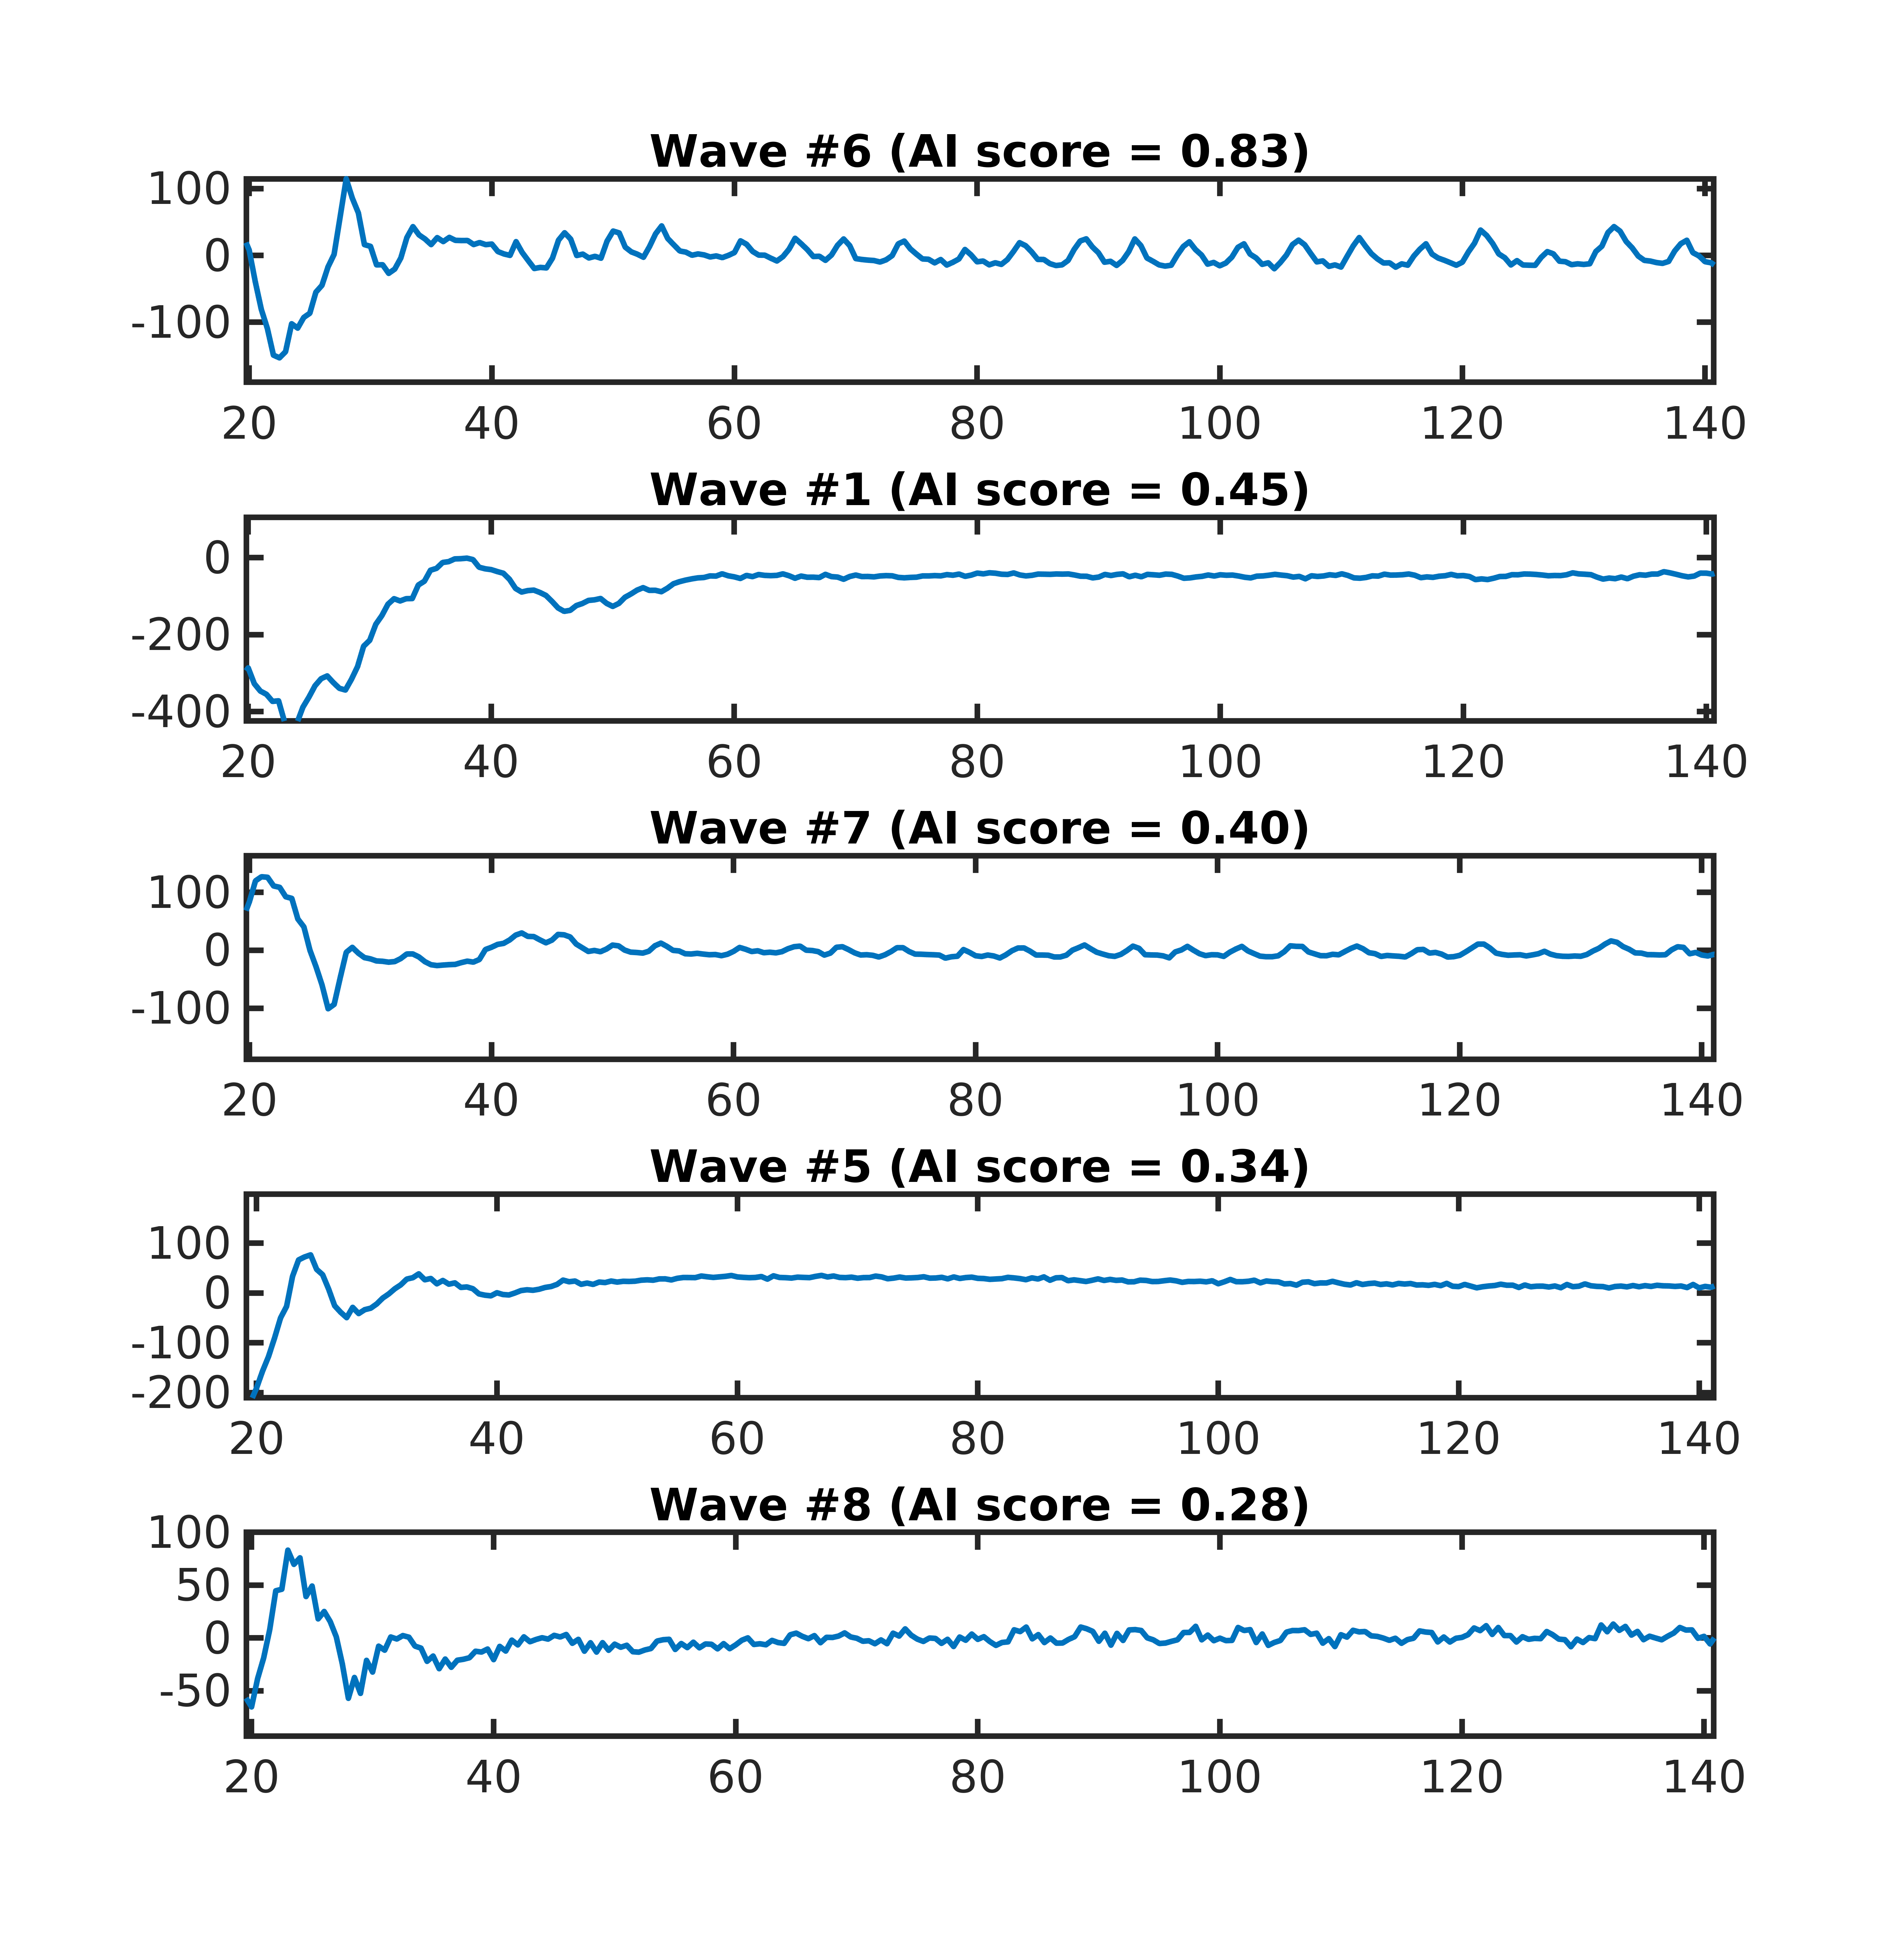
\includegraphics[width=1.0\linewidth]{neural_network_output.png}
                    
                    \captionsetup{singlelinecheck=false}
                    \caption{An example of the output for the \gls{NN} can be seen here testing signals extracted from the first acquisition of patient one using \gls{PCA}.}
                    \label{fig:neural_network_output}
                \end{figure}
                
                A \gls{NN} based scoring metric that was previously developed ~\parencite{Walker2020AutomaticAI}, was tested here to remove complexity and increase robustness when compared to the frequency scoring method. The \gls{NN} of ~\parencite{Walker2020AutomaticAI} is a pretrained model designed to accept a signal as input and return a score between $0.0$ and $1.0$, with a higher score indicating a more respiratory like signal. To achieve this, to avoid issues with signals of different lengths, features of the signal were extracted and used as input to the \gls{NN} (rather than directly inputting the signal itself). For example, one potential feature could be the \gls{PSD} of the signal. The network was trained on scores predetermined by clinicians. Specifically two clinicians scored the signals used to train this model as either being a score of $0.0$, $0.5$, or $1.0$, the mean of the scores from the two clinicians was used as target values. Examples of the output of the \gls{NN} can be seen in figure~\ref{fig:neural_network_output}.
            
            Once a score for each signal has been determined the list of \glspl{PC} is sorted following this scoring as in the algorithm~\ref{alg:score_and_select_pseudo_code}.
        
        \subsubsection{Combine} \label{sec:combine}
            \begin{algorithm} \label{alg:combine_pseudo_code}
                \caption{Combining \glspl{PC}}
                \KwData{\textit{timeSeriesSinograms}, \textit{PCs}}
                \KwResult{\textit{respiratoryPC}}
                \textit{respiratoryPC} = first \gls{PC} in \textit{PCs}\;
                remove \textit{respiratoryPC} from \textit{PCs}\;
                \textit{respiratoryScore} = get score from \textit{respiratoryPC} and \textit{timeSeriesSinograms}\;
                \;
                \For{\gls{PC} in \textit{PCs}}{
                    \textit{currentRespiratoryScore} = get score from \gls{PC} and \textit{timeSeriesSinograms}\;
                    \;
                    \textit{scaledRespiratoryPC} = \textit{respiratoryPC} $\times$ \textit{respiratoryScore}\;
                    \textit{scaledCurrentPC} = \gls{PC} $\times$ \textit{currentRespiratoryScore}\;
                    \;
                    \textit{sumPC} = \textit{scaledRespiratoryPC} + \textit{scaledCurrentPC}\;
                    \textit{subtractPC} = \textit{scaledRespiratoryPC} - \textit{scaledCurrentPC}\;
                    \;
                    \textit{sumRespiratoryScore} = get score from \textit{sumPC} and \textit{timeSeriesSinograms}\;
                    \textit{subtractRespiratoryScore} = get score from \textit{subtractPC} and \textit{timeSeriesSinograms}\;
                    \;
                    \eIf{\textit{sumRespiratoryScore} \textgreater \textit{respiratoryScore}}{
                        \textit{respiratoryPC} = \textit{sumPC}\;
                        \textit{respiratoryScore} = \textit{sumRespiratoryScore}\;
                    }{
                        \uIf{\textit{subtractRespiratoryScore} \textgreater \textit{respiratoryScore}}{
                            \textit{respiratoryPC} = \textit{subtractPC}\;
                            \textit{respiratoryScore} = \textit{subtractRespiratoryScore}\;
                        }
                    }
                }
            \end{algorithm}
            
            After the \glspl{PC} are sorted from high to low score, they are then iterated over, both being summed and subtracted (with a weighting, the score) and a new score is found for both resulting signals. If one of the signals increases, this score then it becomes the new best \gls{PC} and goes forward to the next iteration. \glspl{PC} are both summed and subtracted to handle the arbitrary sign problem mentioned earlier in section~\ref{sec:moving_window_method}~\parencite{Bertolli2017}.
            
            A similar method of combining signals can be seen in~\parencite{Kesner2010AMethods}. However, the method presented here attempts to improve that by using a metric to define a good signal specifically looks to maximise a value related to the behaviour desired, while in~\parencite{Kesner2010AMethods}, the standard deviation is maximised. In addition, the proposed method computes the metric based on signals derived from \glspl{PC} as opposed to single voxel or sinogram bin values, which should lead to noise reduction.
            
            Please note that the algorithm~\ref{alg:combine_pseudo_code} is described in terms of \glspl{PC}. In fact, a simpler version just sums and subtracts the corresponding signals, this will give the same final signal. 
        
            In our current implementation, this method is applied on all time intervals at once. It is possible to integrate this method with the Late Time Interval method in section~\ref{sec:late_time_interval_method} or the Moving Window method. However, this has not been demonstrated here.
            
\section{Evaluation} \label{sec:evaluation}
    \begin{table}
        \centering
        
        \captionsetup{singlelinecheck=false}
        \caption{This table shows the correlation coefficient between the result of the Score, Select, and Combine using \gls{NN} scoring and the \gls{RPM} for the train dataset where a number of pre- and post-processing methods have been applied to the data. Each new line represents the addition of this method, therefore the last time includes all previous pre- and post-processing. This is for the Freeman-Tukey transform, the Yeo-Johnson transform, the incorporation of a mask to remove low count areas of the sinogram, smoothing and downsampling the sinogram and smoothing the signal, and parallel compression.}
        
        \begin{tabular}{||c||c|c||}
            \hline
            \textbf{Correlation Coefficient with RPM}   & \SI{20}{\second}-\SI{840}{\second}    & \SI{20}{\second}-\SI{140}{\second} \\
            \hline
            \hline
            \textbf{Freeman-Tukey}                      & $0.783$                               & $0.703$ \\
            \hline
            \textbf{Yeo-Johnson}                        & $0.790$                               & $0.747$ \\
            \hline
            \textbf{Mask}                               & $0.826$                               & $0.824$ \\
            \hline
            \textbf{Smoothing and Downsampling}         & $0.826$                               & $0.825$ \\
            \hline
            \textbf{Parallel Compression}              & $0.830$                                & $0.839$ \\
            \hline
        \end{tabular}
        \label{tab:pre_and_post_processing_correlation}
    \end{table}
    
    Here, we discuss how the data was prepared for evaluation. We also present a suite of methods which can be applied generally to \glspl{SS} (both from dynamic as well as potentially static acquisitions) in order to combat issues such as noise and outliers. Finally, in this section, we highlight how the methods in section~\ref{sec:methods} will be evaluated in section~\ref{sec:results}.
        
    \subsection{Data Preparation} \label{sec:data_preparation}
        \gls{TOF} data were unlisted into low spatial resolution sinograms, each with a time frame duration of \SI{500}{\milli\second}, using the \gls{GE} PetToolbox, following~\parencite{Bertolli2017DataData}, resulting in sinograms with dimensions $95\times16\times47\times11$ (radial positions$\times$angles$\times$transaxial plane$\times$\gls{TOF}). To extract respiratory variation, the sampling rate of the \gls{PET} sinograms was chosen as \SI{2}{\hertz}, so as to attempt to mitigate the effect of cardiac motion~\parencite{Bertolli2018Data-DrivenTomography}.
        
        Data was pre-processed element-wise by first applying a Freeman-Tukey transformation~\parencite{Freeman1950TransformationsRoot} followed by a Yeo-Johnson power transformation~\parencite{Yeo2000ASymmetry}, to transform the Poisson distributed data to be more Gaussian-like.

        In the current implementation, these transformations are applied element-wise on the (Poisson distributed) \gls{TOF} sinogram $S_p$
        
        \begin{equation} \label{eq:freeman_tukey_yeo_johnson}
            S_g = \mathrm{YJ_\lambda}(\mathrm{FT}(S_p))
        \end{equation}

        The Freeman-Tukey transformation is defined as
        
        \begin{equation} \label{eq:freeman_tukey}
            \mathrm{FT}(X) = \sqrt{X + 1} + \sqrt{X}
        \end{equation}
        
        The Yeo-Johnson power transformation is defined as
        
        \begin{equation} \label{eq:yeo_johnson}
            \mathrm{YJ_\lambda}(X) =   \begin{cases}
                        ((X + 1)^\lambda - 1) / \lambda                   & \quad \text{if } \lambda \neq 0 \text{, } X \geq 0 \\
                        \log(X + 1)                                       & \quad \text{if } \lambda = 0 \text{, } X \geq 0    \\
                        -[(-X + 1)^{(2 - \lambda)} - 1)] / (2 - \lambda)  & \quad \text{if } \lambda \neq 2 \text{, } X < 0    \\
                        -\log(-X + 1)                                     & \quad \text{if } \lambda = 2 \text{, } X < 0
                    \end{cases}
        \end{equation}
        
        The $\lambda$ parameter is determined by minimising the \gls{KLD} between normal distributions and the transformed distribution~\parencite{Yeo2000ASymmetry}. In this paper a single $\lambda$  was determined from all of the data, although it would be feasible to find different $\lambda$ values for every element in the sinogram.

        The impact of including the Yeo-Johnson power transformation can be seen in table~\ref{tab:pre_and_post_processing_correlation}.
        
        It was previously found through experimentation that Gaussian smoothing of the resulting sinograms can improve results, especially in the case of the \gls{SAM} methods~\parencite{Thielemans2013ComparisonData}. In the current implementation, further downsampling was performed post-smoothing to reduce memory usage and increase computational speed. Linear interpolation was used as it was shown in a preliminary investigation to give satisfactory results at little computational cost. Although block reduction (by summing patches of data of size four or eight etc) is more computationally efficient and may potentially have benefits with regards to noise over linear interpolation. However, block reduction is limited in what downsampling factors can be used while interpolation is not. We use linear interpolation here to reduce the matrix size to a size necessary to represent the highest frequency information present in the data post-smoothing. The effect this inclusion makes on the end result can be seen in table~\ref{tab:pre_and_post_processing_correlation}.
        
        Finally, it has been found that the introduction of a mask to further aid in the reduction of noise is beneficial~\parencite{Thielemans2011}. The mask itself is defined as being true for any value, in the sinogram, above a predetermined threshold. Values not in the mask are removed prior to further execution, this is because these values can be assumed to mostly be noise. Note that a mask can also be used to eliminate parts of the data potentially affected by non-respiratory movement~\parencite{Bertolli2018Data-DrivenTomography}, but this has not been implemented in the current work. Again, the impact of this inclusion can be seen in table~\ref{tab:pre_and_post_processing_correlation}.

        Values for the Gaussian smoothing and the threshold of the mask were determined using a grid search on a randomly selected subset of the data (specifically three patients), this data was then not used as part of any final evaluation as was stated in section~\ref{sec:data_acquisition_and_train_test_split}. The Gaussian smoothing sigma for the \gls{PCA} based methods were $1.0$, $0.5$, and $2.0$, for \gls{SAM} based methods they were $1.0$, $3.0$, and $1.0$ for the sinogram radial positions, angles, and transaxial planes respectively. The mask threshold is selected programmatically such that it removes the bottom \SI{5}{\percent} of values. The same mask is used for every time point. From an examination of the masks used for the test dataset, because a threshold value as low as \SI{5}{\percent} is used, it appears that the mask is only removing parts of the background.

    \subsection{Post-Processing} \label{sec:post_processing}
        Regardless of the method used there are still some effects of the radiotracer kinetics to be expected at early time intervals and noise throughout. Thus a method is proposed here to aid with the remaining radiotracer kinetics and smoothing to help with noise in the extracted \gls{SS}. The same post-processing is used regardless of the method to extract the \gls{SS}.
            
        \subsubsection{Parallel Compression} \label{sec:parallel_compression}   
            Firstly there is, what shall be referred to as ``parallel compression''. This is a method borrowed from audio engineering (appearing notably in Dolby A noise reduction). The signal is split into two channels, one has its dynamic range reduced (through a process such as compression) while the other passes unchanged before they are averaged back together~\parencite{Izhaki2012MixingTools}. This has the effect of reducing large differences in the dynamic range of the signal (for instance caused by tracer kinetics or some kind of drift) without losing a lot of breath to breath variability compared to directly using the phase of the signal (if applied to respiratory surrogate signals)~\parencite{Lamare2022PETVadis}. For a more detailed explanation of the implementation please see the appendix.

        \subsubsection{Outlier Removal} \label{sec:outlier_removal}
            Even though most of the large changes in intensity are remedied by parallel compression, some momentary spikes are still apparent. Thus, outliers are removed where they are outside a threshold of the quartile of the signal and new values are interpolated.

        \subsubsection{Smoothing} \label{sec:smoothing}
            Finally, smoothing is applied through the use of a bandpass filter (specifically a sinc filter) followed by a Savitzky-Golay filter~\parencite{Savitzky1964SmoothingProcedures}. A bandpass filter is used to remove frequencies in the signal outside of the respiratory window and the Savitzky-Golay filter is used to promote local smoothness.

            The bandpass filter is defined as

            \begin{equation} \label{eq:bandpass_filter}
                h_{BPF}(t) = 2B_Hsinc(2B_Ht) - 2B_Lsinc(2B_Lt)
            \end{equation}

            \noindent where in equation~\ref{eq:bandpass_filter} $h_{BPF}$ is the bandpass function, $t$ is the time distributed variable, $B_H$ is the upper bound and $B_L$ is the lower bound of the bandpass filter. The bandpass filter is implemented using a truncated sinc kernel. A polynomial order of three and a window length of five was used with the Savitzky-Golay filter determined through a grid search on the training dataset.

        The impact of the inclusion of the above methods on the correlation of the Select, Score, and Combine method with \gls{NN} based scoring with the \gls{RPM} can be seen in table~\ref{tab:pre_and_post_processing_correlation}.

    \subsection{Evaluation Methods} \label{sec:evaluation_methods}        
        For evaluation of the results, the correlation coefficient of each surrogate signal between each method and the \gls{RPM}, for all acquisitions in the test dataset, has been calculated. The correlation coefficient has been calculated for both the first \SI{120}{\second} (ignoring the first \SI{20}{\second}) and also the entire acquisition (between \SI{20}{\second} and \SI{840}{\second}). A statistical analysis using a mixed effects model has also been included.
        
        All methods were compared to conventional \gls{PCA}. We also included results for the Moving Window \gls{SAM} method as this approximates \gls{KRG}.
        While the Conventional and Late Time Interval methods can also be implemented using \gls{SAM}, corresponding results are not shown here.

        As stated earlier in section~\ref{sec:data_acquisition_and_train_test_split}, parameters for the methods have been selected using a grid search on a randomly selected subset of the data (specifically three patients), this data was then not used as part of any final evaluation. The parameters were optimised by maximising the correlation coefficient between the surrogate signal and the \gls{RPM} for the first \SI{120}{\second} of usable data (between \SI{20}{\second} and \SI{140}{\second}) due to there being initially no counts in the \gls{FOV}.
            
\section{Results} \label{sec:results}
    \begin{figure}
        \centering
        
        \includegraphics[width=1.0\linewidth]{patient_one_baseline_output.png}
        
        \captionsetup{singlelinecheck=false}
        \caption{Output of each method compared to the \gls{RPM} for the first usable \SI{120}{\second} (between \SI{20}{\second} and \SI{140}{\second}) (taken for the first acquisition of patient one). This is for Conventional \gls{PCA}, Moving Window \gls{PCA}, Late Time Interval \gls{PC}, Score, Select, and Combine using frequency and \gls{NN} scoring, and the Moving Window \gls{SAM} method.}
        \label{fig:patient_one_baseline_output}
    \end{figure}
    
    \begin{figure}
        \centering
        
        \includegraphics[width=1.0\linewidth]{patient_eight_baseline_output.png}
        
        \captionsetup{singlelinecheck=false}
        \caption{Output of each method compared to the \gls{RPM} for the first usable \SI{120}{\second} (between \SI{20}{\second} and \SI{140}{\second}) (taken for the first acquisition of patient eight). This is for Conventional \gls{PCA}, Moving Window \gls{PCA}, Late Time Interval \gls{PC}, Score, Select, and Combine using frequency and \gls{NN} scoring, and the Moving Window \gls{SAM} method.}
        \label{fig:patient_eight_baseline_output}
    \end{figure}

    \begin{figure}
        \centering
        
        \includegraphics[width=1.0\linewidth]{box_plot_early.png}
        
        \captionsetup{singlelinecheck=false}
        \caption{A box plot showing for each method its correlation coefficient to the \gls{RPM} for the first usable \SI{120}{\second} (between \SI{20}{\second} and \SI{140}{\second}) (taken for the seven test acquisitions). This is for Conventional \gls{PCA}, Moving Window \gls{PCA}, Late Time Interval \gls{PC}, Score, Select, and Combine using frequency and \gls{NN} scoring, and the Moving Window \gls{SAM} method.}
        \label{fig:box_plot_early}
    \end{figure}

    \begin{figure}
        \centering
        
        \includegraphics[width=1.0\linewidth]{box_plot_all.png}
        
        \captionsetup{singlelinecheck=false}
        \caption{A box plot showing for each method its correlation coefficient to the \gls{RPM} for the entire acquisition (taken for the seven test acquisitions). This is for Conventional \gls{PCA}, Moving Window \gls{PCA}, Late Time Interval \gls{PC}, Score, Select, and Combine using frequency and \gls{NN} scoring, and the Moving Window \gls{SAM} method.}
        \label{fig:box_plot_all}
    \end{figure}

    \begin{figure}
        \centering
        
        \includegraphics[width=1.0\linewidth]{pca_signals.png}
        
        \captionsetup{singlelinecheck=false}
        \caption{Signals for the first usable \SI{120}{\second} (between \SI{20}{\second} and \SI{140}{\second}) generated using the Select, Score, and Combine \gls{NN} based scoring method. This is for the five acquisitions which did not have a usable \gls{RPM} signal and as such could not be used for training or testing.}
        \label{fig:pca_signals}
    \end{figure}
    
    \begin{figure}
        \centering
        
        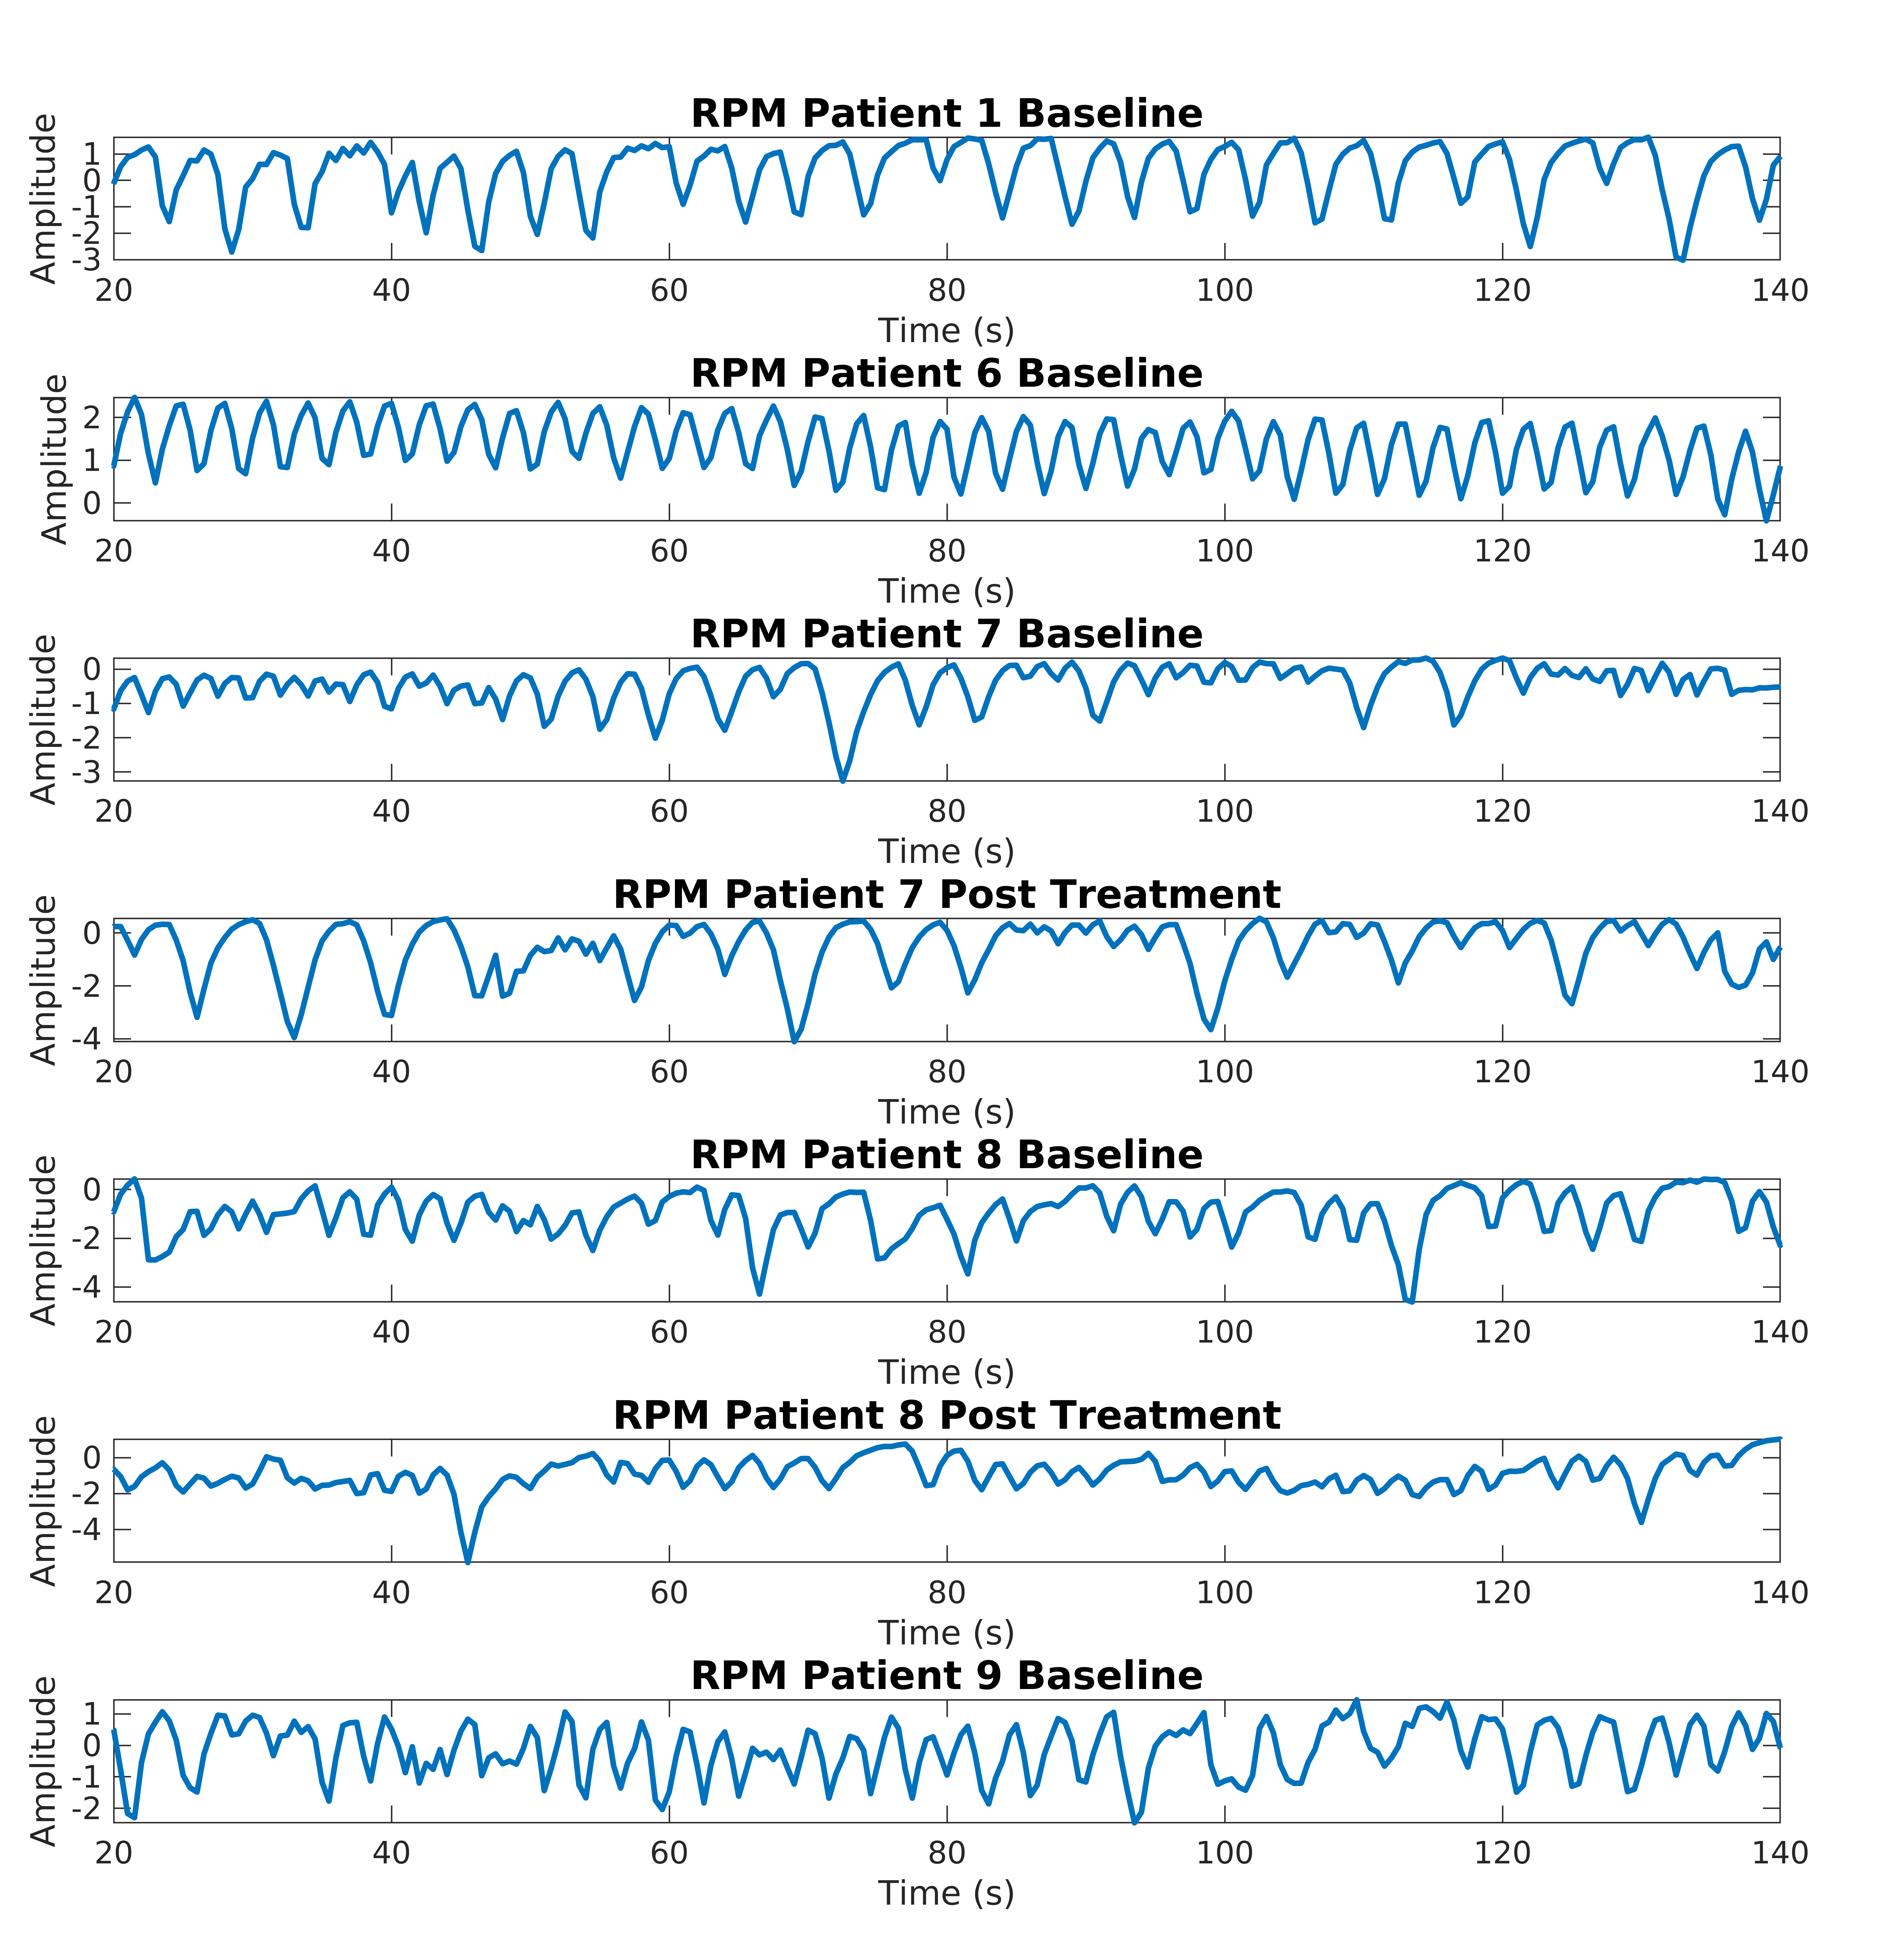
\includegraphics[width=1.0\linewidth]{rpm_signals.png}
        
        \captionsetup{singlelinecheck=false}
        \caption{\gls{RPM} signals for the first usable \SI{120}{\second} (between \SI{20}{\second} and \SI{140}{\second}) (for the seven test acquisitions). Notice that only the first acquisition of patient one and patient six shows a steady trace with an average frequency, every other trace shows variable breathing or artefacts.}
        \label{fig:rpm_signals}
    \end{figure}

    \begin{figure}
        \centering
        
        \includegraphics[width=1.0\linewidth]{rpm_spectral_density.png}
        
        \captionsetup{singlelinecheck=false}
        \caption{The result of applying \gls{FFT} to the \gls{RPM} signals for the first usable \SI{120}{\second} (between \SI{0.05}{\hertz} and \SI{0.45}{\hertz}) (for the seven test acquisitions). Notice that four of the seven have peaks very close to or outside the lower boundary of the resiratory window. Also notice that two of the seven have very wide frequency responses, which would be difficult for the automatic selection of a respiratory frequency window.}
        \label{fig:rpm_spectral_density}
    \end{figure}
    
    \begin{figure}
        \centering
        
        \includegraphics[width=1.0\linewidth]{all_correlation_coefficient.png}
        
        \captionsetup{singlelinecheck=false}
        \caption{Correlation coefficients to the \gls{RPM} for the first \SI{120}{\second} in \SI{20}{\second} intervals (between \SI{20}{\second} and \SI{140}{\second}) (taken as a mean for all data sets). This is for Conventional \gls{PCA}, Moving Window \gls{PCA}, Late Time Interval \gls{PC}, Score, Select, and Combine using frequency and \gls{NN} scoring, and the Moving Window \gls{SAM} method. The stair plots are staggered for the different methods for visual clarity.}
        \label{fig:all_cross_correlation}
    \end{figure}
    
    \begin{figure}
        \centering
        
        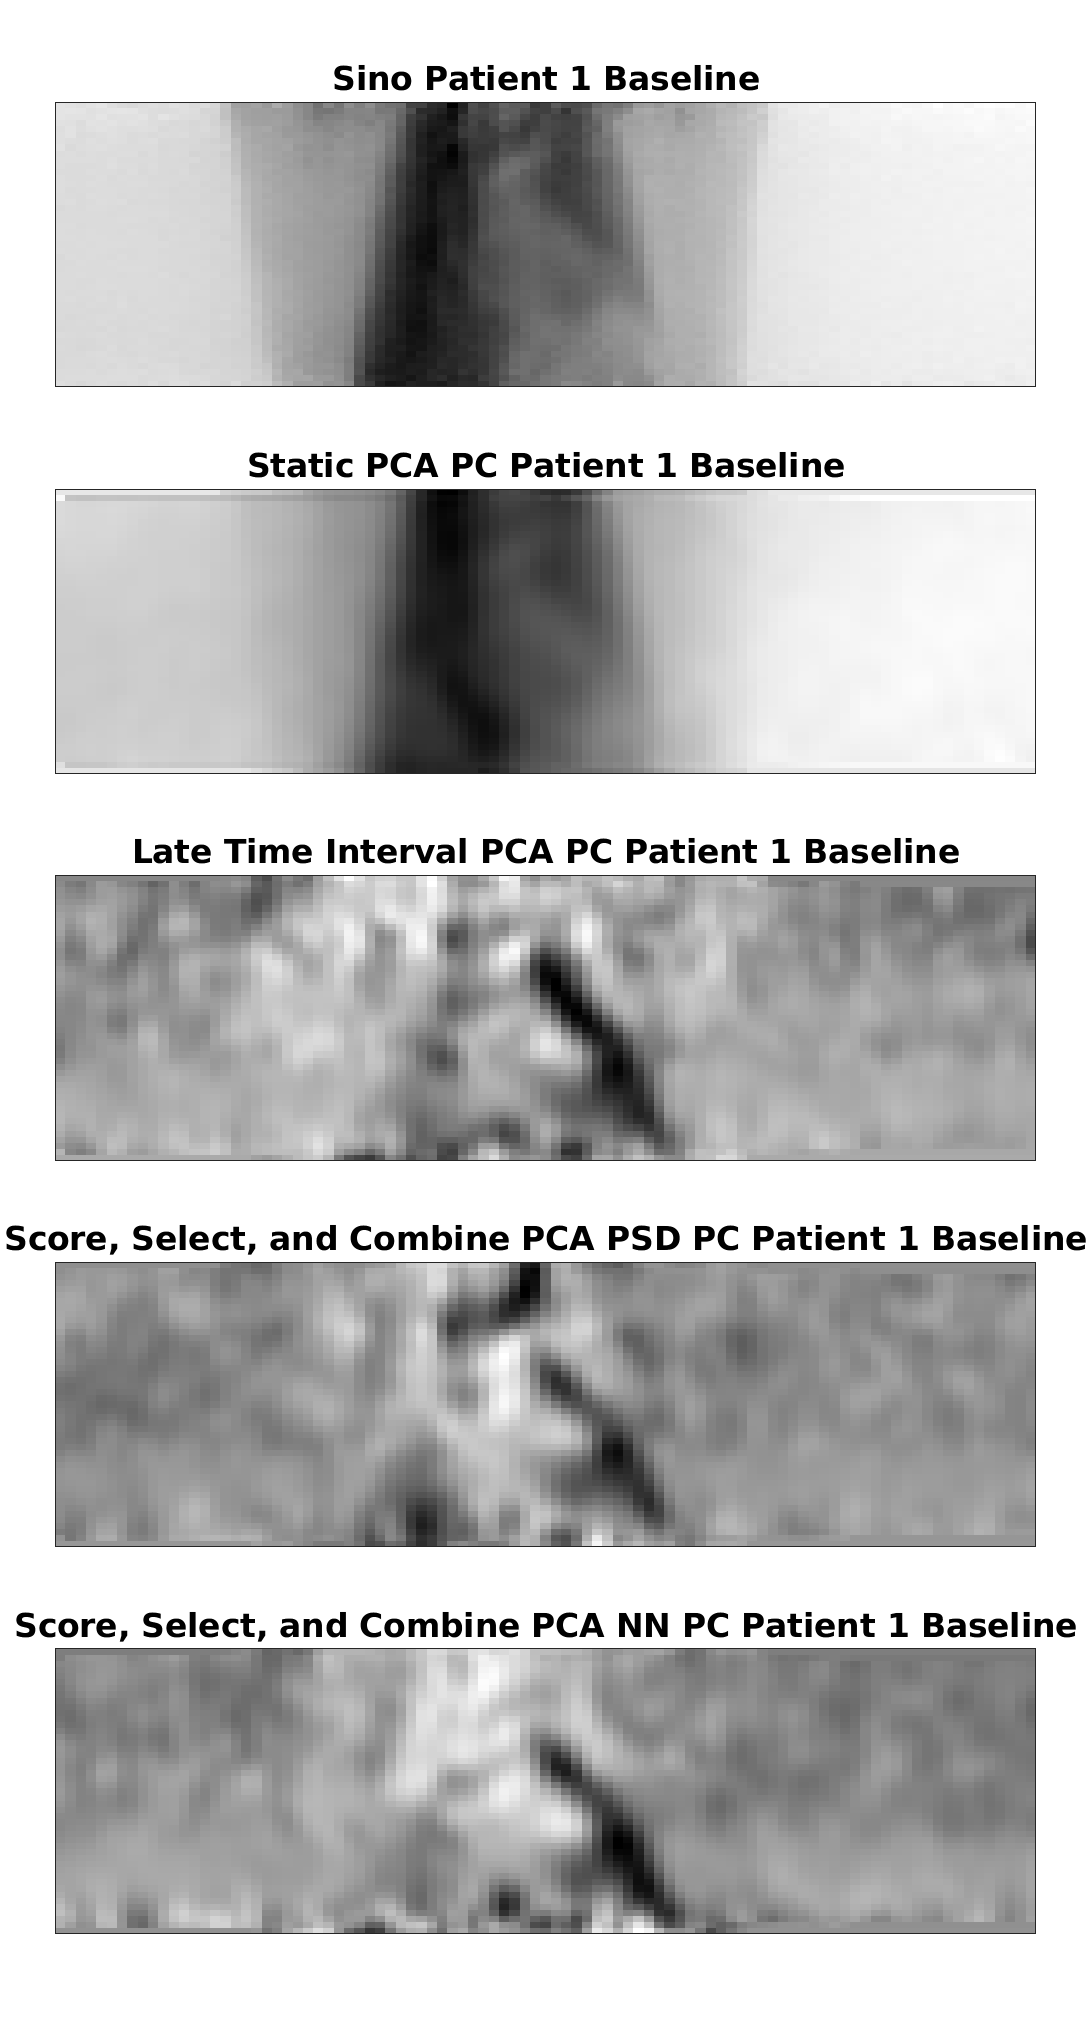
\includegraphics[width=0.7\linewidth]{patient_one_pc_output.png}
        
        \captionsetup{singlelinecheck=false}
        \caption{A plot showing a single `view' of the original PET data (top) as well as the \glspl{PC} used to generate the output signal for the Conventional, Late Time Interval and the two Score, Select, and Combine methods (taken for the first acquisition of patient one).}
        \label{fig:patient_one_pc_output}
    \end{figure}

    \begin{table}
        \centering
        
        \captionsetup{singlelinecheck=false}
        \caption{This table shows the p-values acquired as part of a statistical analysis of the test dataset using a mixed-effects model. Before applying the mixed-effects model the signals were first transformed to frequency space using \gls{FFT}. One values between \SI{0.05}{\hertz} and \SI{0.45}{\hertz} were used. This is for Conventional \gls{PCA}, Moving Window \gls{PCA}, Late Time Interval \gls{PC}, Score, Select, and Combine using frequency and \gls{NN} scoring, and the Moving Window \gls{SAM} method.}
        
        \begin{tabular}{||c||c||}
            \hline
            \textbf{Mixed-Effects Model}                & \textbf{p-value} \\
            \hline
            \hline
            \textbf{Static PCA}                         & $0.183$ \\
            \hline
            \textbf{Moving Window PCA}                  & $0.483$ \\
            \hline
            \textbf{Late Time Interval PCA}             & $0.548$ \\
            \hline
            \textbf{Score, Select, and Combine PCA PSD} & $0.649$ \\
            \hline
            \textbf{Score, Select, and Combine PCA NN}  & $0.908$ \\
            \hline
            \textbf{Moving Window SAM}                  & $0.373$ \\
            \hline
        \end{tabular}
        \label{tab:statistical_analysis}
    \end{table}
    
    A plot showing for each method its output compared to the \gls{RPM} for the first \SI{120}{\second} (between \SI{20}{\second} and \SI{140}{\second}) (taken for the first acquisition of patient one) can be seen in figure~\ref{fig:patient_one_baseline_output}. From a visual analysis, it can be observed that the Conventional \gls{PCA} method has failed. Post normalisation it appears almost as if there is no variation in the signal at early time intervals. Both moving window methods show towards the end of the plot that they can extract a signal, however it takes until between \SI{60}{\second} and \SI{80}{\second} for both methods to begin to pick up the signal. For the \gls{SAM} based method it appears as if the sign determination method has failed before \SI{80}{\second}, regardless though the method still cannot extract a signal before \SI{60}{\second}. The Late Time Interval \gls{PC}, Score, Select, and Combine using frequency and \gls{NN} scoring methods all appear to be able to extract a usable signal right down to \SI{20}{\second} (around when counts begin to appear in the \gls{FOV}). The magnitude of the signal post \SI{80}{\second} more closely matches the \gls{RPM} (or in comparison to before \SI{80}{\second}) for both Select and Combine methods than for the Late Time Interval \gls{PC} method.
    
    A plot showing for each method its output compared to the \gls{RPM} for the first \SI{120}{\second} (between \SI{20}{\second} and \SI{140}{\second}) (taken for the first acquisition of patient eight) can be seen in figure~\ref{fig:patient_eight_baseline_output}. Similar results as for in figure~\ref{fig:patient_one_baseline_output} are repeated in figure~\ref{fig:patient_eight_baseline_output}, although all methods match the \gls{RPM} worse than in figure~\ref{fig:patient_one_baseline_output}. This acquisition was selected to be shown due to it being a difficult trace to extract. Regardless, the Late Time Interval \gls{PC} and Select and Combine methods appear to have extracted a signal early into the acquisition (from about \SI{35}{\second} on this patient and acquisition).
    
    A box plot showing for each method its correlation coefficient to the \gls{RPM} for both the first \SI{120}{\second} (between \SI{20}{\second} and \SI{140}{\second}) and also for the entire acquisition (taken for seven acquisitions) can be seen in figure~\ref{fig:box_plot_early} and figure~\ref{fig:box_plot_all}. The correlation coefficient for the Conventional \gls{PCA} method is low and the method is not usable. The correlation coefficients for both the moving window methods are roughly around $0.5$, indicating  that the Moving Window method is beneficial regardless of the method used to extract the signal for each window. However, again here the correlation coefficient is lower than is acceptable. The results from the Late Time Interval \gls{PC}, Score, Select, and Combine using frequency and \gls{NN} scoring methods all show correlation coefficients around $0.6$ or higher for both the early time interval as well as for all data. The Score, Select, and Combine methods show marginally higher correlation coefficient than the Late Time Interval \gls{PC} method and the \gls{NN} shows slightly higher correlation coefficient than the frequency based scoring.
    
    A plot showing for each method the evolution of the correlation coefficient with the \gls{RPM} over time for the first \SI{120}{\second} by computing it in \SI{20}{\second} intervals can be seen in figure~\ref{fig:all_cross_correlation}. It can be observed that on average across all data sets all methods struggle to produce usable results at the very beginning of the acquisition (around when counts begin to appear in the \gls{FOV}). However, it is also apparent that on average both Score, Select, and Combine methods robustly begin to produce results which closely match the \gls{RPM}, as evidenced by a reasonable correlation past the first \SI{40}{\second} on most acquisitions. The Moving Window method appears to perform well in the first interval.
    
    A plot showing the component (or their combination) used to generate the output signal can be seen in figure~\ref{fig:patient_one_pc_output}. One advantage of the sinogram-based methods is that the \gls{PC} (or signed mask for \gls{SAM}) can be visualised to see how it corresponds to anatomy and tracer uptake. In figure~\ref{fig:patient_one_pc_output} it can be seen that the Conventional \gls{PCA} method returns a \gls{PC} which closely resembles the input data, leading to the conclusion that the variation in the selected \gls{PC} is dominated by the kinetics. The other methods produce a \gls{PC} which is more related to edges of internal structures where respiratory movement occurs. A visual inspection indicates that the least confounding variation and noise is included in the Score, Select, and Combine method using the \gls{NN} scoring method. Curiously it appears that the Late Time Interval and the Score, Select, and Combine method using the \gls{NN} scoring method return very similar distributions. However, the Score, Select, and Combine method using the frequency scoring method also returns a high value region in tissue at the top of the image.

    We utilised a mixed-effects model to analyse the differences between various methods and \gls{RPM} measurements across all subjects. This model incorporated `method' as a fixed effect and treated subjects as a random effect to account for inter-subject variability. We found that the comparisons between each method and \gls{RPM} were not statistically significant, with all p-values $> 0.05$, see table~\ref{tab:statistical_analysis}. While this may suggests that, within the constraints of our analysis and available data, there was no evidence to support significant differences between any methods in comparison to \gls{RPM} measurements, given the small number of subjects, it's important to consider that this analysis may be considerably underpowered. 

    It is noteworthy to mention that we observed that the Late Time Interval \gls{PC}, Score, Select, and Combine using frequency and \gls{NN} scoring methods exhibited the highest p-values, which may suggest a lesser degree of difference from \gls{RPM}. However, such interpretations should be approached with caution and not be taken as conclusive evidence of similarity.

    Finally, results of applying the Score, Select, and Combine using \gls{NN} scoring method to data where the \gls{RPM} could not by synced with the list mode data can be seen in~\ref{fig:pca_signals}.
    
\section{Discussion} \label{sec:discussion}
    This paper introduces several methods for \gls{DD} extraction of a respiratory signal from dynamic \gls{PET} data. To the best of our knowledge, this appears to have only been attempted in~\parencite{Schleyer2014}. Data used here are from a \gls{18F-FDG} study on patients with \gls{IPF}, while in the latter paper, \gls{13N-NH3} data was used to evaluate the proposed \gls{KRG} method.
    
    The work presented here suffers from several limitations. Firstly, the data used here all originates from the same study, using the same procedure, the same radiotracer, and acquired on the same scanner. In order to better validate the generalisability of the method it would be positive to test on data acquired on different scanners and using different radiotracers. Additionally, from the data acquired only a subset of this data is usable due to issues during acquisition, the number of participants is limited. It would be beneficial to test the methods on a larger sample of patients, with both a larger number of non-complex and complex breathers to better test the limitations of the methods.
    
    An additional concern is the point at which the methods may fail for patients who exhibit abnormal breathing patterns. For instance, extremely slow breathers will breathe at a rate less than \SI{0.1}{\hertz}, which in the case of the Score, Select, and Combine method using the frequency scoring method and a fixed frequency respiratory window would be considered to be radiotracer kinetics. Furthermore, when using a non-fixed respiratory window this method struggles with patients who breathe less regularly as the window is expanded to include parts of the kinetics and noise (this is shown in figure~\ref{fig:rpm_spectral_density}). The discrepancy between the results for the \gls{SAM} Moving Window method, presented here, and the \gls{KRG} ones shown in~\parencite{Schleyer2014} could also be attributed to this complexity. Many of the patients breathed at varying rates, stopped breathing during acquisition, or breathed unusually fast or slow (this is shown in figure~\ref{fig:rpm_signals}). This was probably due to the data being acquired for an \gls{IPF} study.

    The presented method includes several pre- and post-processing steps. Although these have been shown to be beneficial on the train data, table~\ref{tab:pre_and_post_processing_correlation}, the impact of some steps is relatively small. It remains to be determined on a larger dataset if some of these steps could be removed.

    A limitation of the concept of using \glspl{SS} at all in the pursuit of the motion correction of respiratory motion is the transform from a \gls{1D} \gls{SS} to the \gls{3D} motion. There are methods, such as one using a \gls{MM} parameterised by the \gls{SS}~\parencite{McClelland2017, McClelland2013}. However, they are not trivial, and in the case where a \gls{1D} \gls{SS} is used, limit breath to breath variability and hysteresis to being periodic~\parencite{Whitehead2021ComparisonMap}. There are beginning to be methods for motion correction which are conditioned on features of the acquisition rather than a \gls{SS}~\parencite{Huang2023Surrogate-DrivenData, Huang2024Surrogate-drivenData}.
    
\section{Conclusion} \label{sec:conclusion}
    We have presented and evaluated several methods for extraction of a respiratory signal from dynamic \gls{PET} data. Results from a visual comparison of early time interval output signals compared to the \gls{RPM}, quality of \gls{PC} and correlation coefficient of the output signals to the \gls{RPM} indicates that the Late Time Interval \gls{PC} and both Score, Select, and Combine methods are more robust and afford higher quality signals than moving window methods. The results also indicate that both Score, Select, and Combine methods can give a higher correlation coefficient earlier than the Late Time Interval \gls{PC} method and that scoring using the \gls{NN} shows slightly higher correlation coefficients than the frequency based scoring.

    In the future, research will focus on further development of the method, including optimisation of the \gls{NN} scoring method. In the next stage, these methods will be applied to the task of implementing advanced respiratory motion correction on dynamic \gls{PET} data.

\section*{Appendix} \label{sec:appendix}
    \subsection*{Parallel Compression} \label{appendix:parallel_compression}
        \begin{figure}
            \centering
            
            \includegraphics[width=1.0\linewidth]{parallel_compression_weighting.png}
            
            \captionsetup{singlelinecheck=false}
            \caption{This figure shows an example of the processed count rate and processed gradient of the processed count rate, between \SI{0}{\second} and \SI{140}{\second}, which are used as part of the parallel compression post-processing step. These have been taken for the first acquisition of patient one. Here the processed count rate is normalised between zero and one by subtracting by the minimum and dividing by the maximum value of the signal.}
            \label{fig:parallel_compression_weighting}
        \end{figure}

        \begin{algorithm} \label{alg:parallel_compression_pseudo_code}
            \caption{Parallel Compression}
            \KwData{\textit{timeSeriesSinograms}, \textit{respiratorySignal}, \textit{windowSize}}
            \KwResult{\textit{respiratorySignal}}
            \For{\textit{index} in length of \textit{timeSeriesSinograms} - \textit{windowSize}}{
                \;
                \textit{currentRespiratorySignal} = \textit{respiratorySignal} for data between \textit{index} and \textit{index} + \textit{windowSize}\;
                \;
                \textit{currentRespiratorySignal} = \textit{currentRespiratorySignal} - mean of \textit{currentRespiratorySignal}\;
                \textit{currentRespiratorySignal} = $\dfrac{\textit{currentRespiratorySignal}}{\mathrm{standard \ deviation\ of\ }\textit{currentRespiratorySignal}}$\;
                \;
                \textit{windowSignal} = fill with \glspl{NaN} to \textit{index}\;
                \textit{windowSignal} append \textit{currentRespiratorySignal}\;
                \textit{windowSignal} append \glspl{NaN} to length of \textit{timeSeriesSinograms}\;
                \;
                \textit{respiratorySignals} append \textit{windowSignal}\;
                \;
            }
            \;
            \textit{lowDynamicRangeSignal} = mean of \textit{signals} ignoring \glspl{NaN}\;
            \;
            \textit{weighting} = get weighting from \textit{timeSeriesSinograms}\;
            \;
            \textit{lowDynamicRangeSignal} = \textit{lowDynamicRangeSignal} $\times$ \textit{weighting}\;
            \textit{respiratorySignal} = \textit{respiratorySignal} $\times$ ($1$ - \textit{weighting})\;
            \;
            \textit{respiratorySignal} = \textit{respiratorySignal} + \textit{lowDynamicRangeSignal}\;
        \end{algorithm}

        \begin{algorithm} \label{alg:extract_parallel_compression_weighting_pseudo_code}
            \caption{Extract Parallel Compression Weighting}
            \KwData{\textit{timeSeriesSinograms}}
            \KwResult{\textit{processedGradientOfProcessedCountRate}}
            \For{\textit{sinogram} in \textit{timeSeriesSinograms}}{
                \textit{countRate} append sum of \textit{sinogram}\;
            }
            \;
            \textit{processedCountRate} = moving average of \textit{countRate}\;
            \;
            \textit{gradientOfProcessedCountRate} = gradient of \textit{processedCountRate}\;
            \;
            \textit{processedGradientOfProcessedCountRate} = absolute of \textit{processedGradientOfProcessedCountRate}\;
            \;
            \textit{processedGradientOfProcessedCountRate} = reverse of \textit{processedGradientOfProcessedCountRate}\;
            \textit{currentMaximumValue} = 0.0\;
            \;
            \For{\textit{value} in \textit{processedGradientOfProcessedCountRate}}{
                \eIf{\textit{value} \textgreater \textit{currentMaximumValue}}{
                    \textit{currentMaximumValue} = \textit{value}\;
                }{
                    \textit{value} = \gls{NaN}\;
                }
            }
            \;
            \textit{processedGradientOfProcessedCountRate} = reverse of \textit{processedGradientOfProcessedCountRate}\;
            linear interpolate \glspl{NaN} in \textit{processedGradientOfProcessedCountRate}\;
            \;
            \textit{processedGradientOfProcessedCountRate} = centred moving average of \textit{processedGradientOfProcessedCountRate}\;
            \;
            \textit{processedGradientOfProcessedCountRate} = \textit{processedGradientOfProcessedCountRate} - minimum of \textit{processedGradientOfProcessedCountRate}\;
            \textit{processedGradientOfProcessedCountRate} = $\dfrac{\textit{processedGradientOfProcessedCountRate}}{maximum\ of\ \textit{processedGradientOfProcessedCountRate}}$\;
        \end{algorithm}

        This appendix contains a detailed description of what is presented breifly in section~\ref{sec:parallel_compression}. This method attempts to limit the dynamic range of a signal proportionally in time to how much that signal is expected to be affected by artefacts. The signal is duplicated into two channels and one of these channels is then split temporally into a series of small moving windows. These windows are \SI{20}{\second} in size and overlap by their length minus one (the stride size is one). The values in each window are then standardised independently, the windows are averaged back together, before being combined with the unadulterated channel following the weighting seen in figure~\ref{fig:parallel_compression_weighting}. An example of the algorithm can be seen in the algorithm~\ref{alg:parallel_compression_pseudo_code}.
        
        The channels are combined following the gradient of the count rate. An example of the signals involved can be seen in figure~\ref{fig:parallel_compression_weighting} and an example of the algorithm can be seen in the algorithm~\ref{alg:extract_parallel_compression_weighting_pseudo_code}.

        \begin{itemize}
            \item Firstly, the count rate over time is found by summing all elements of each sinogram. A moving average smoothing is then applied to this processed count rate signal with a size of \SI{5}{\second}.
            
            \item Secondly, the gradient of the processed count rate is taken. The absolute of this signal is used, as we are interested in the change in gradient (but not the direction). Next the processed gradient of the processed count rate signal is iterated over from its last value to its first, if the value decreases it is replaced by interpolation using the previous value and the next value that is larger than the previous value. Finally a (centred) moving average smoothing is applied to the signal with a size of \SI{20}{\second}, and the signal is normalised between zero and one by subtracting by the minimum and dividing by the maximum value of the signal.
            
            \item Thirdly, the low and high dynamic range respiratory signals are summed using the magnitude of the processed gradient of the processed count rate signal as a weighting. At time intervals where the magnitude of the processed count rate signal is greater, more of the compressed/standardised signal is summed compared to the non-compressed/non-standardised signal. The total weighting is always equal to one, to maintain the scale. To achieve this, the low dynamic range respiratory signal is multiplied directly by the processed gradient of the processed count rate signal and the high dynamic range respiratory signal is multiplied by one minus the processed count rate signal (before both respiratory signals are summed together).
        \end{itemize}

    % \section*{Acknowledgments}
    %     This research was supported by GE Healthcare, the NIHR UCLH Biomedical Research Centre and the UCL EPSRC Centre for Doctoral Training in Intelligent, Integrated Imaging in Healthcare (i4health) grant (EP/L016478/1).
        
    %     The software used was partly produced by the Computational Collaborative Project on Synergistic Biomedical Imaging, CCP SyneRBI, UK EPSRC grant (EP/T026693/1).
        
    %     Jamie~R.~McClelland is supported by a Cancer Research UK Centres Network Accelerator Award grant (A21993) to the ART-NET consortium and a CRUK Multi-disciplinary grant (CRC 521).
    
    \printbibliography
\end{document}
